\documentclass{VUMIFPSkursinis}
\usepackage{algorithmicx}
\usepackage{algorithm}
\usepackage{algpseudocode}
\usepackage{amsfonts}
\usepackage{amsmath}
\usepackage{booktabs}
\usepackage{blindtext}
\usepackage{bm}
\usepackage{caption}
\usepackage{color}
\usepackage{colortbl}
\usepackage{float}
\usepackage{graphicx}
\usepackage{listings}
\usepackage{multirow}
\usepackage{scrextend}
\usepackage{subfig}
\usepackage{wrapfig}
\usepackage{longtable}
\usepackage{enumitem}
\usepackage{xparse}
%\usepackage{tabularx}
\usepackage{ltxtable}
\usepackage{tabu}
\usepackage{xcolor}

% Titulinio aprašas
\university{Vilniaus universitetas}
\faculty{Matematikos ir informatikos fakultetas}
\department{Matematikos ir informatikos institutas}
\papertype{Testavimo atvejai ir rasti defektai}
\title{Programos ,,Christmas Time Calculator" testavimas}
\status{3 kurso 5 grupės studentė}
\author{Gabrielė Saletytė}
\supervisor{dr. Vytautas Valaitis}
\date{Vilnius – \the\year}

% Nustatymai
% \setmainfont{Palemonas}   % Pakeisti teksto šriftą į Palemonas (turi būti įdiegtas sistemoje)
\bibliography{bibliography}

\colorlet{headcolor}{gray!25}
\renewcommand{\tabularxcolumn}[1]{ m{#1} }
\newcommand\TopSpace{\rule{0pt}{2.6ex}}       % Top strut
\newcommand\BottomSpace{\rule[-1.2ex]{0pt}{0pt}} % Bottom strut
\newcolumntype{M}[1]{ >{\centering\arraybackslash} m{#1} }

\newcounter{subCount}
\newcounter{ir}
\setcounter{ir}{0}
\newcounter{fr}
\setcounter{fr}{0}
\newcounter{nfr}
\setcounter{nfr}{0}

\newcommand{\ir}[2]{%
    \stepcounter{ir}
    \generateTable{IR\their}{#1}{#2}
}

\newcommand{\fr}[2]{%
    \stepcounter{fr}
    \generateTable{FR\thefr}{#1}{#2}
}

\newcommand{\nfr}[2]{%
    \stepcounter{nfr}
    \generateTable{NFR\thenfr}{#1}{#2}
}

\makeatletter
\def\nobreakhline{%
  \noalign{\ifnum0=`}\fi
    \penalty\@M
    \futurelet\@let@token\LT@@nobreakhline}
\def\LT@@nobreakhline{%
  \ifx\@let@token\hline
    \global\let\@gtempa\@gobble
    \gdef\LT@sep{\penalty\@M\vskip\doublerulesep}% <-- change here
  \else
    \global\let\@gtempa\@empty
    \gdef\LT@sep{\penalty\@M\vskip-\arrayrulewidth}% <-- change here
  \fi
  \ifnum0=`{\fi}%
  \multispan\LT@cols
     \unskip\leaders\hrule\@height\arrayrulewidth\hfill\cr
  \noalign{\LT@sep}%
  \multispan\LT@cols
     \unskip\leaders\hrule\@height\arrayrulewidth\hfill\cr
  \noalign{\penalty\@M}%
  \@gtempa}
\makeatother

\newcommand{\header}[1]{%
    \nobreakhline
    \multicolumn{3}{|c|}{\cellcolor{headcolor} #1} \\*
    \nobreakhline
}

\newcommand{\generateTable}[3]{%
    #1 &
    {
        \setcounter{subCount}{1}%
        \let\oldbackslash\\
        \renewcommand{\tabularxcolumn}[1]{ p{##1} }%
        \begin{tabularx}{\linewidth}{  @{\hspace{\tabcolsep}#1.\thesubCount\ifnum\value{subCount}<10 \hphantom{0}\fi\hspace{\tabcolsep}} | X  }
          \global\def\\{\TopSpace\BottomSpace\stepcounter{subCount}\oldbackslash \hline}
          #3
        \end{tabularx}%
        \global\let\\\oldbackslash
    } &
    #2 \\
    \hline
}

%==========================================================================> Dokumento pradžia <========================================================================
\begin{document}
    \newenvironment{innerParagraph}[1][0.5cm]{\begin{adjustwidth}{#1}{}}{\end{adjustwidth}}
        
    \pagenumbering{gobble}
    \maketitle
    \tableofcontents
	\pagenumbering{arabic}
	
	\sectionnonum{Anotacija} \label{anotacija}
		Šiame laboratoriniame darbe bus testuojama „Christmas Time Calculator“ programa.
		Ši programėlė skirstoma į dvi dalis - pagrindinę, kurią sudaro laiko iki Kalėdų skaičiuoklė, bei papildomą - 
		kurią sudaro kalėdinis žaidimas.
		Sudarant testavimo atvejus bus atsižvelgtą į atskirus dalių funkcionalumus.
		Ši programa rašyta 2016 m. rugsėjo - gruodžio mėn. ir atsiskaityta kaip taikomojo objektinio programavimo užduotis.
		Programa rašyta C\# kalba.

		Pradžioje bus apibrėžti reikalavimai programai, pagal kuriuos buvo atliekama užduotis.
		Vėliau bus pateikiami testavimo atvejai ir sudaryta atsekamumo matrica.
		Laboratorinio darbo pabaigoje bus pateiktas defektų sąrašas ir sudarytas terminų žodynėlis.
	\sectionnonum{Įvadas} \label{ivadas}
		\subsection*{Testuojamos programos pavadinimas} \label{ivadas_psPavadinimas}
			,,Christmas Time Calculator''.
		\subsection*{Darbo tikslas} \label{ivadas_darboTikslas}
			Panaudojant testavimo atvejų sudarymo strategiją rankiniu būdu, 
			ištestuoti „Christmas Time Calculator“ programą, sudaryti testavimo atvejus bei defektų sąrašus.
		\subsection*{Darbo pagrindas} \label{ivadas_pagrindas}
			Dokumentas parengtas kaip programų sistemų testavimo laboratorinis darbas.
	
	\section{Reikalavimai programai ,,Christmas Time Calculator"} \label{reikalavimai}
		Šiame skyriuje pateikiami reikalavimai, į kuriuos buvo atsižvelgiama rašant „Christmas Time Calculator“ programą.
		Reikalavimai pateikiami bendrai, neišskiriant atskirų programos dalių funkcionalumų.
		\begin{enumerate}[label=\textbf{R\arabic*}]
			\item Pagrindiniame programos lange turi būti galimybė keisti „Until Christmas Left“ teksto spalvą paspaudus ant šio užrašo.
			Pasirinkta spalva turi išlikti išjungus programą.
			\item Pagrindiniame lange pasikeitus mėnesių, dienų, valandų, minučių ar sekundžių skaičiui į 1, 
			šalia esantis žodis iš daugiskaitos turi
			pasikeisti į vienaskaitą.
			\item Likus kiekvienai minutei mažiau (t. y. programa rodo 0 ties sekundžių skiltimi), naujame lange įsijungia kalėdinis žaidimas.
			\item Keičiant pagrindinės dalies dydį, visi laukai proporcingai pakeičia savo dydį. 
			Kalėdinio žaidimo lango dydžio keisti nėra galimybės.
			\item Esant įjungtam kalėdiniam žaidimui ir vėl atėjus laikui įjungti jį, žaidimas neįsijungia iš naujo ir 
			nėra atidaromas papildomas langas su nauju žaidimu.
			\item Žaidimo metu su kepurėle pagavus dovanėlę taškai padidėja vienu vienetu.
			Pasiekus naują rekordinį taškų kiekį, skaičius ties „High Score“ nuolat atnaujinamas į dabar surinktų taškų kiekį.
			\item Kalėdinės kepurėlės judėjimas pagrįstas rodyklių bei klavišų „A“ ir „D“ valdymu.
			\item Dovanėlei nukritus iš matomo lauko, prarandama viena gyvybė tai pašalinus vieną iš 3 dovanėlių ikonų.
			\item Krentančios kalėdinės dovanėlės turi būti pilnai matomos žaidimo erdvėje. 
			Dovanėlės negali kristi už matymo ribų ir negali matytis tik dalinai.
			\item Ilgėjant žaidimo laikui, dovanėlių bei kalėdinės kepurėlės judėjimo greičiai proporcingai didėja.
			\item Praradus visas gyvybes, žaidimas turi išsijungti po 5 sekundžių.
			Prieš išsijungiant ekrane turi pasirodyti „Game Over“ užrašas.
			Jei žaidimo metu pasiektas naujas rekordas, vietoj „Game Over“ užrašo turi pasirodyti „New High Score!“ užrašas. 
		\end{enumerate}
	\section{Programos ,,Christmas Time Calculator" testavimas} \label{testavimas}
		Šiame skyriuje bus pateikiami testavimo atvejai bei reikalavimų - testavio atvejų atsekamumo matrica.
		\subsection{Testavimo atvejai} \label{testavimoAtvejai}
			Šioje dalyje pateikiamos lentelės su atskirais testavimo atvejais.
			\subsubsection{Pagrindinės dalies testavimo atvejai} \label{pagrindinesDaliesTA}
				Toliau 1 - 10 lentelėse pateikiami testavimo atvejai, apimantys pagrindinės dalies funkcionalumą.
				\begin{table}[H]
					\centering
					\caption{Užrašo „Until Christmas Left“ teksto spalvos pakeitimo testavimo atvejis}
					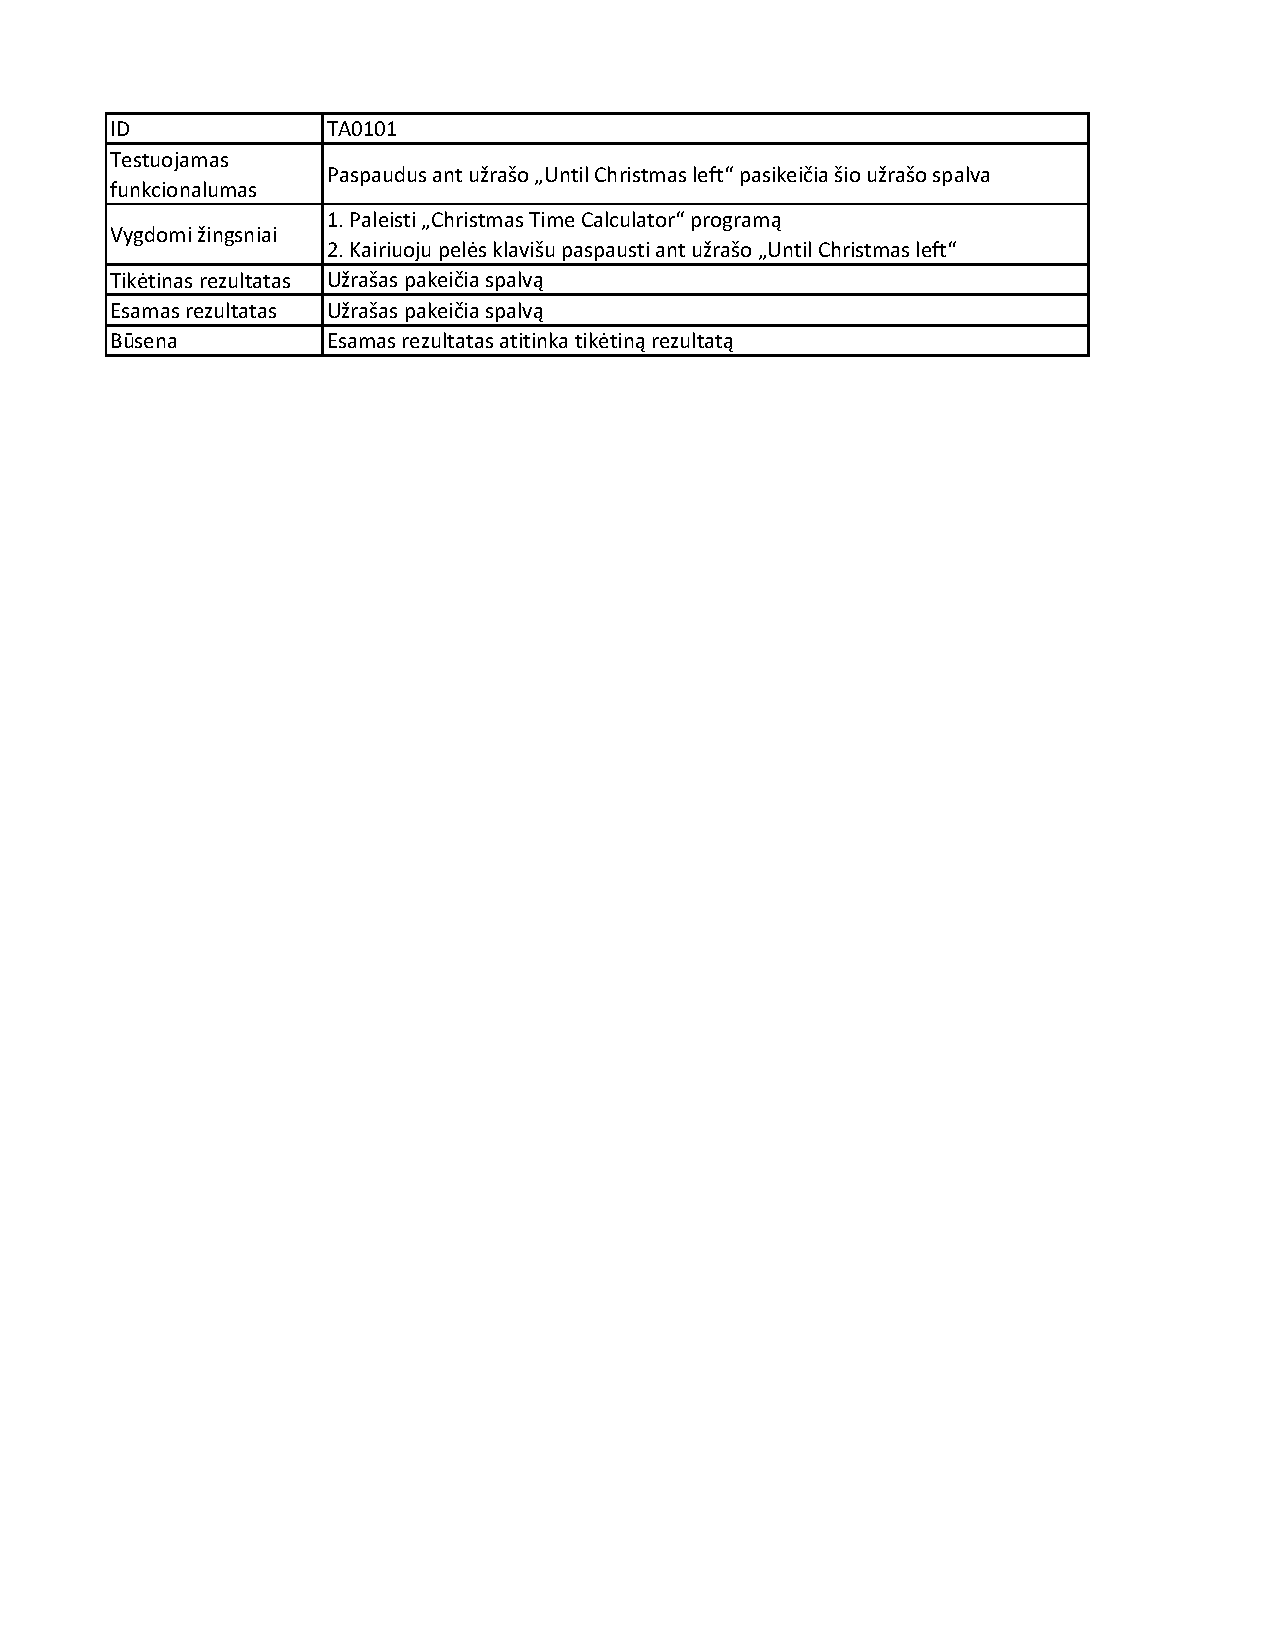
\includegraphics[width=\textwidth]{TA/TA0101}			
					\label{fig:TA0101}
				\end{table}
				\begin{table}[H]
					\centering
					\caption{Užrašo „Until Christmas Left“ teksto spalvos išsaugojimo}
					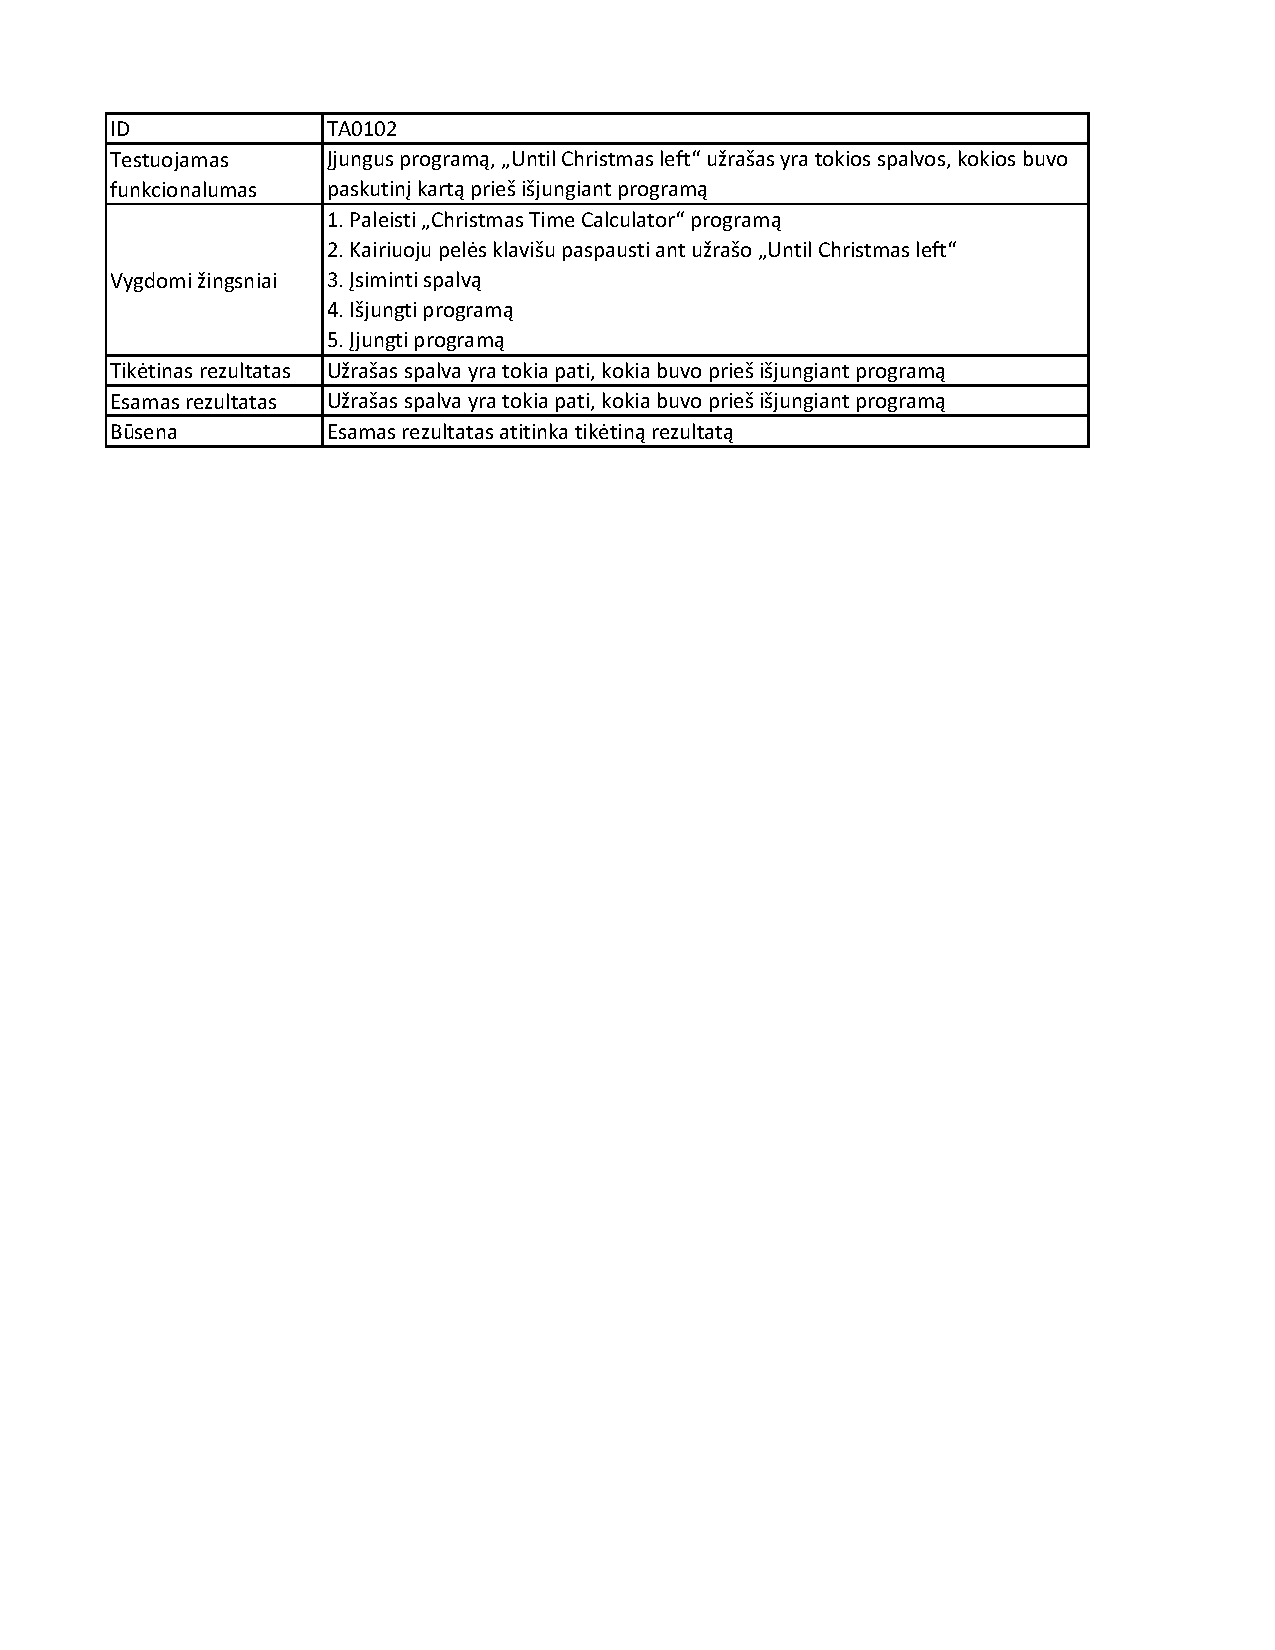
\includegraphics[width=\textwidth]{TA/TA0102}			
					\label{fig:TA0102}
				\end{table}
				\begin{table}[H]
					\centering
					\caption{Mėnesio laukelio teisingumo testavimo atvejis}
					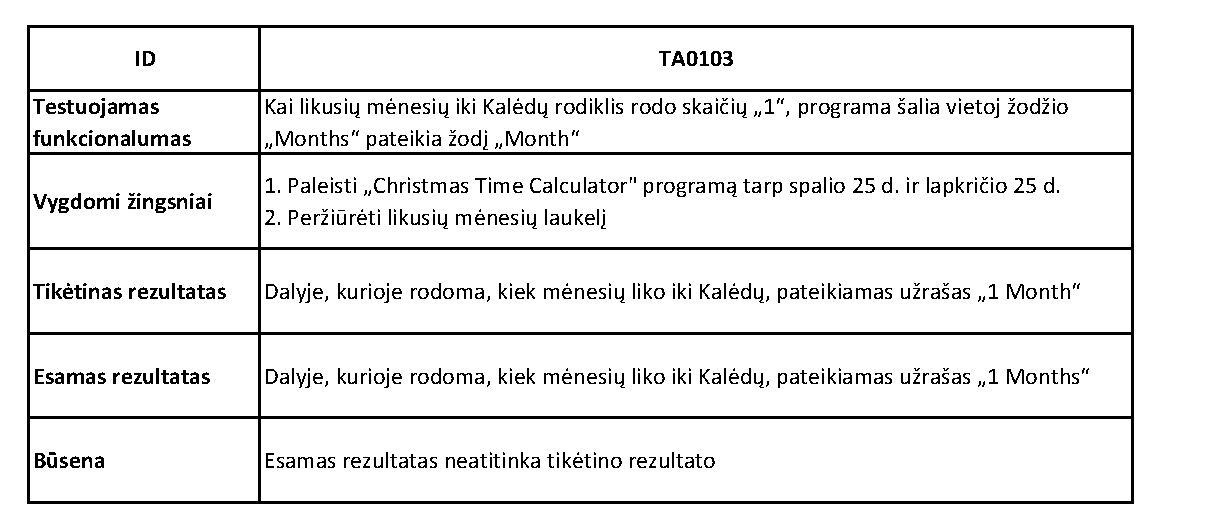
\includegraphics[width=\textwidth]{TA/TA0103}			
					\label{fig:TA0103}
				\end{table}
				\begin{table}[H]
					\centering
					\caption{Dienų laukelio teisingumo testavimo atvejis}
					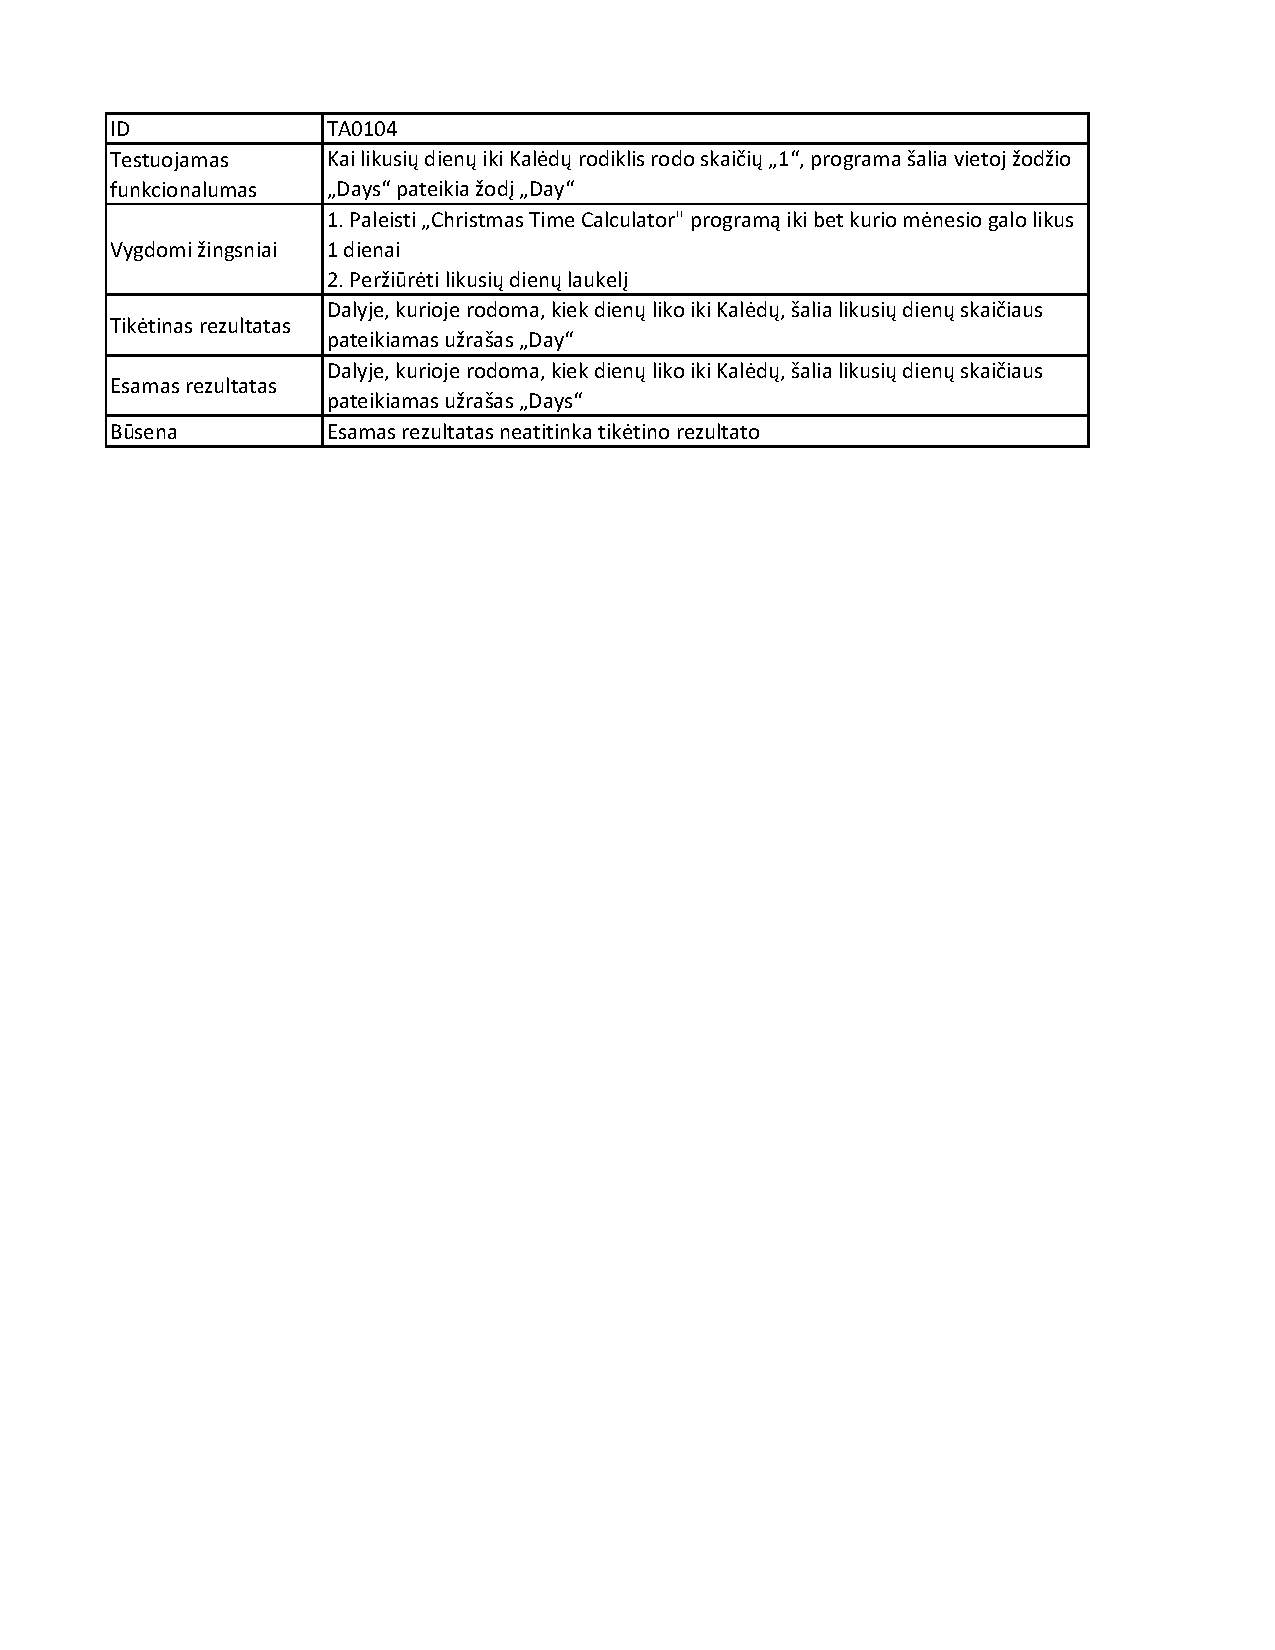
\includegraphics[width=\textwidth]{TA/TA0104}			
					\label{fig:TA0104}
				\end{table}
				\begin{table}[H]
					\centering
					\caption{Valandų laukelio teisingumo testavimo atvejis}
					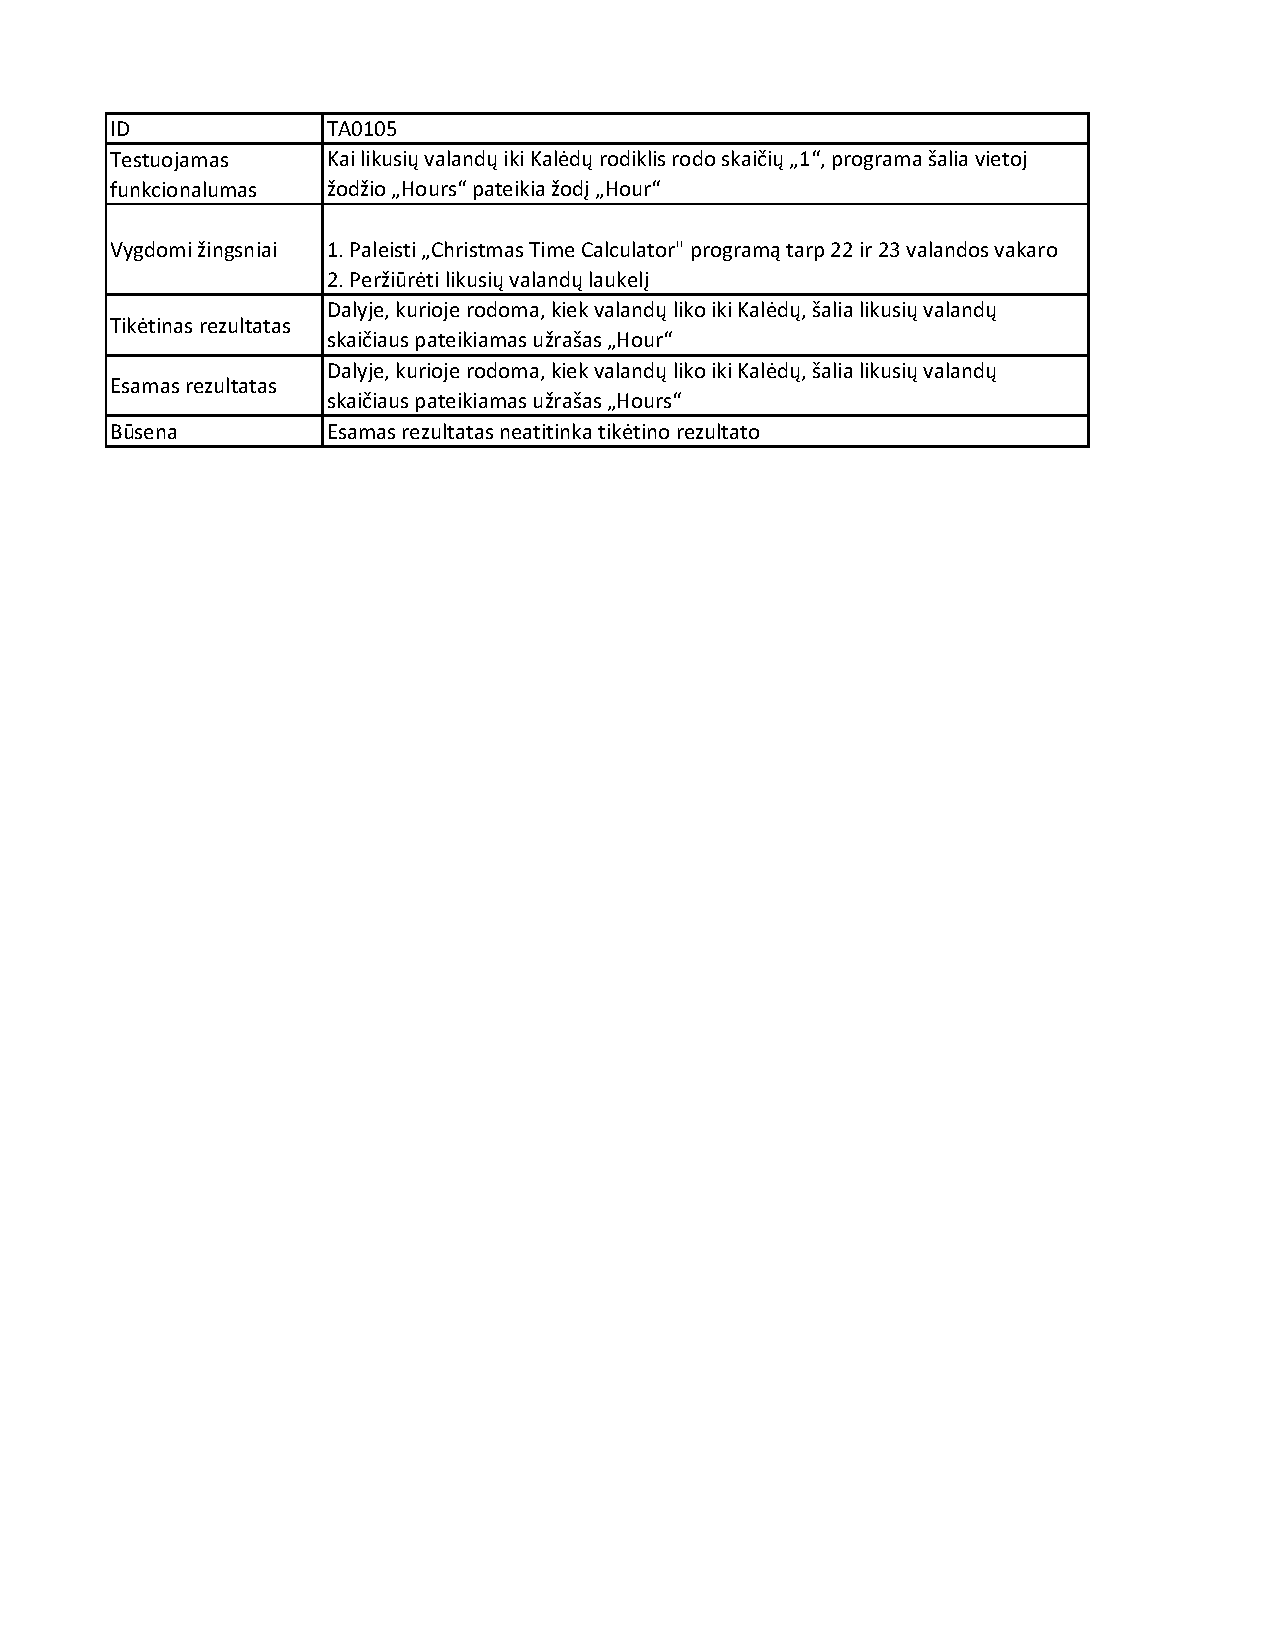
\includegraphics[width=\textwidth]{TA/TA0105}			
					\label{fig:TA0105}
				\end{table}
				\begin{table}[H]
					\centering
					\caption{Minučių laukelio teisingumo testavimo atvejis}
					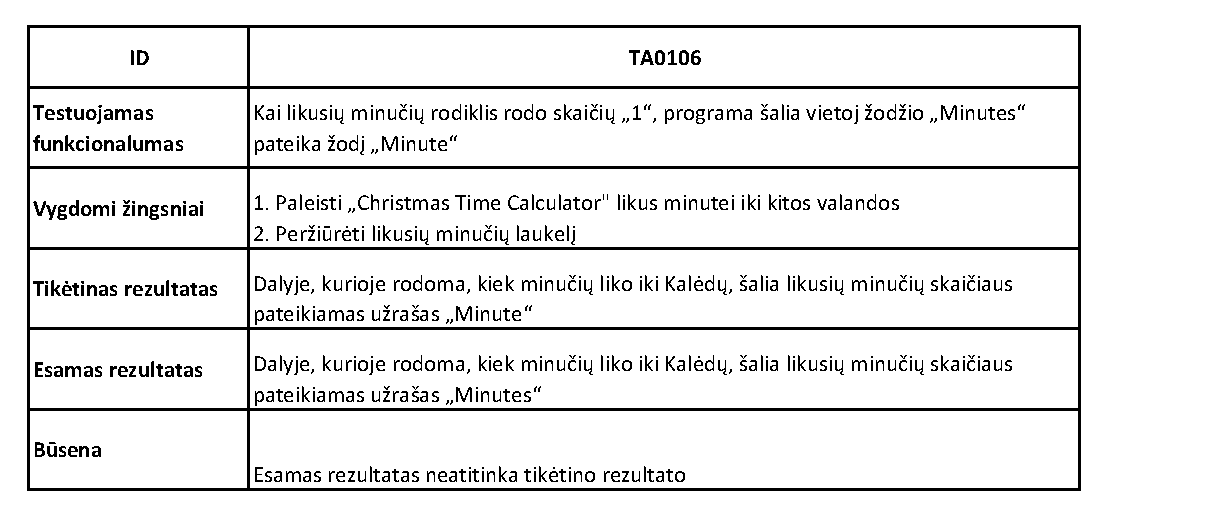
\includegraphics[width=\textwidth]{TA/TA0106}			
					\label{fig:TA0106}
				\end{table}
				\begin{table}[H]
					\centering
					\caption{Sekundžių laukelio teisingumo testavimo atvejis}
					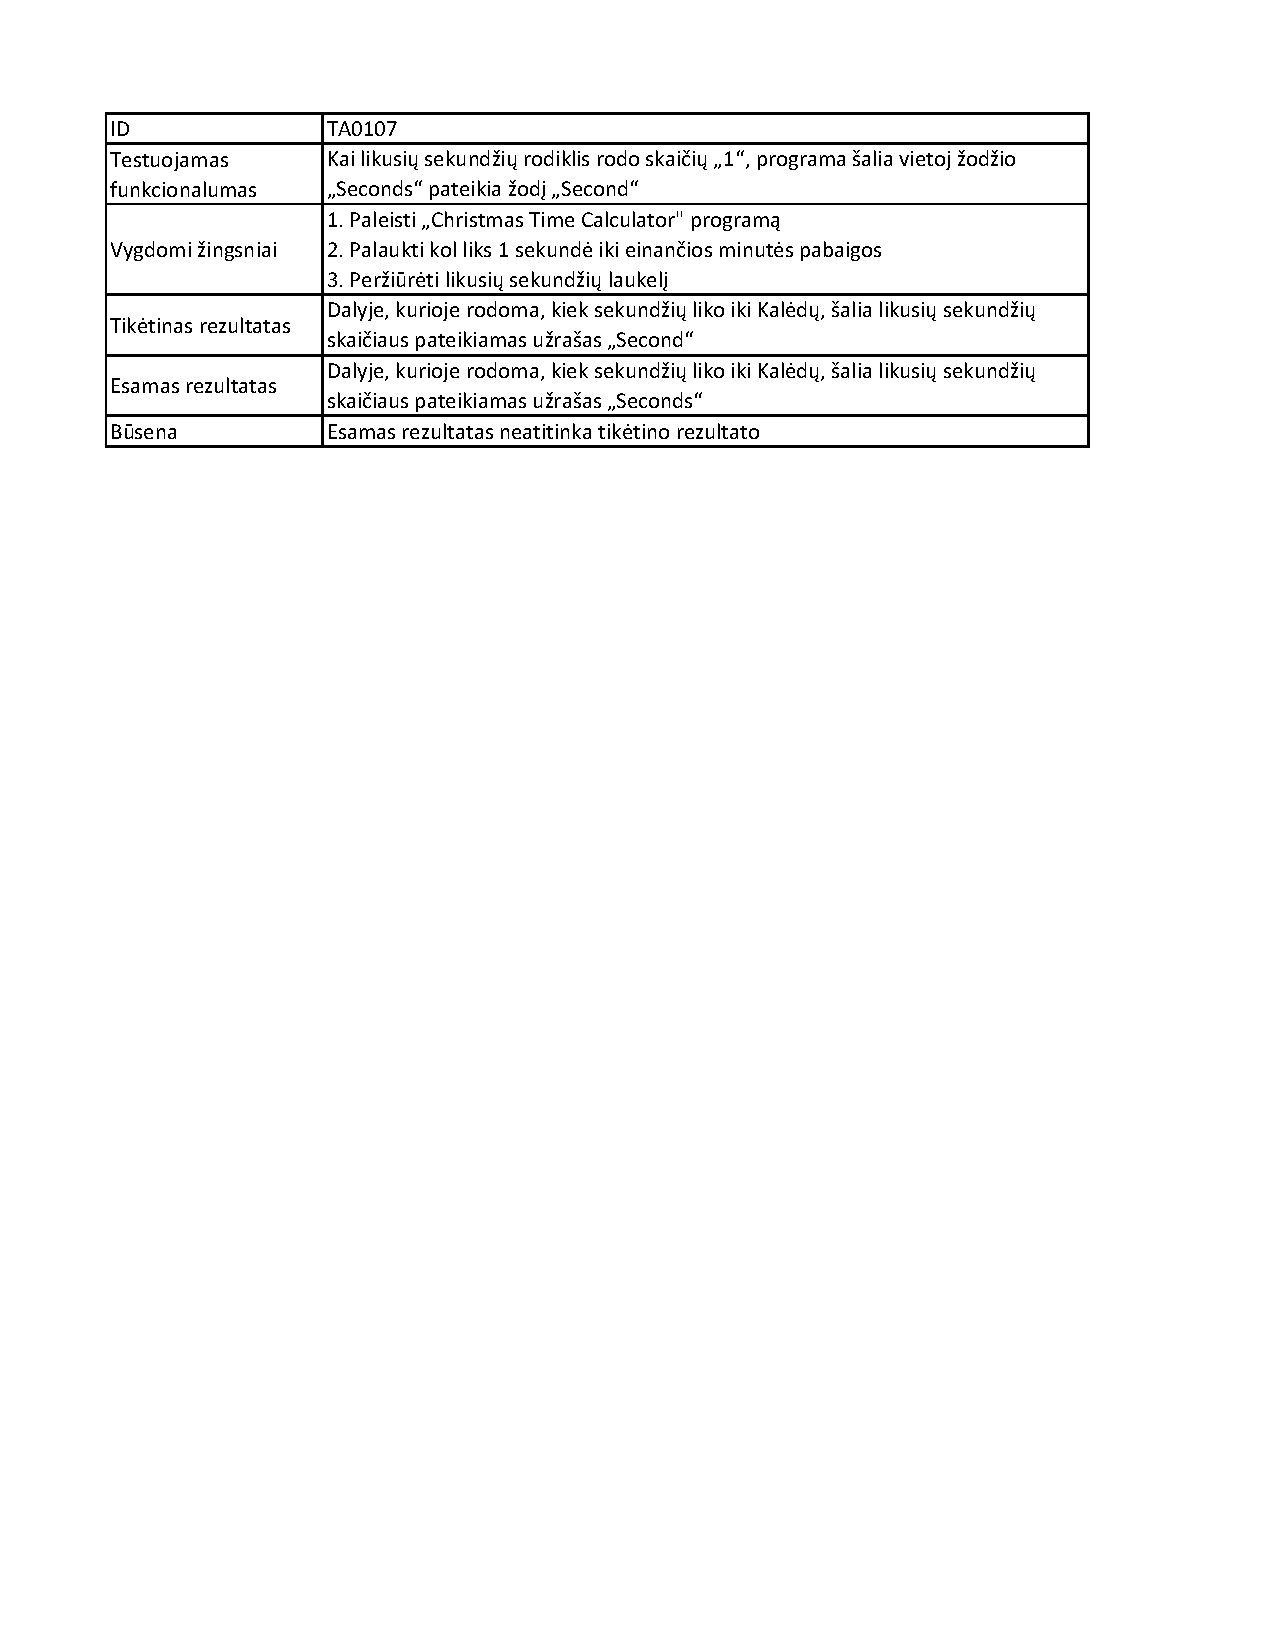
\includegraphics[width=\textwidth]{TA/TA0107}			
					\label{fig:TA0107}
				\end{table}
				\begin{table}[H]
					\centering
					\caption{Žaidimo paleidimo testavimo atvejis}
					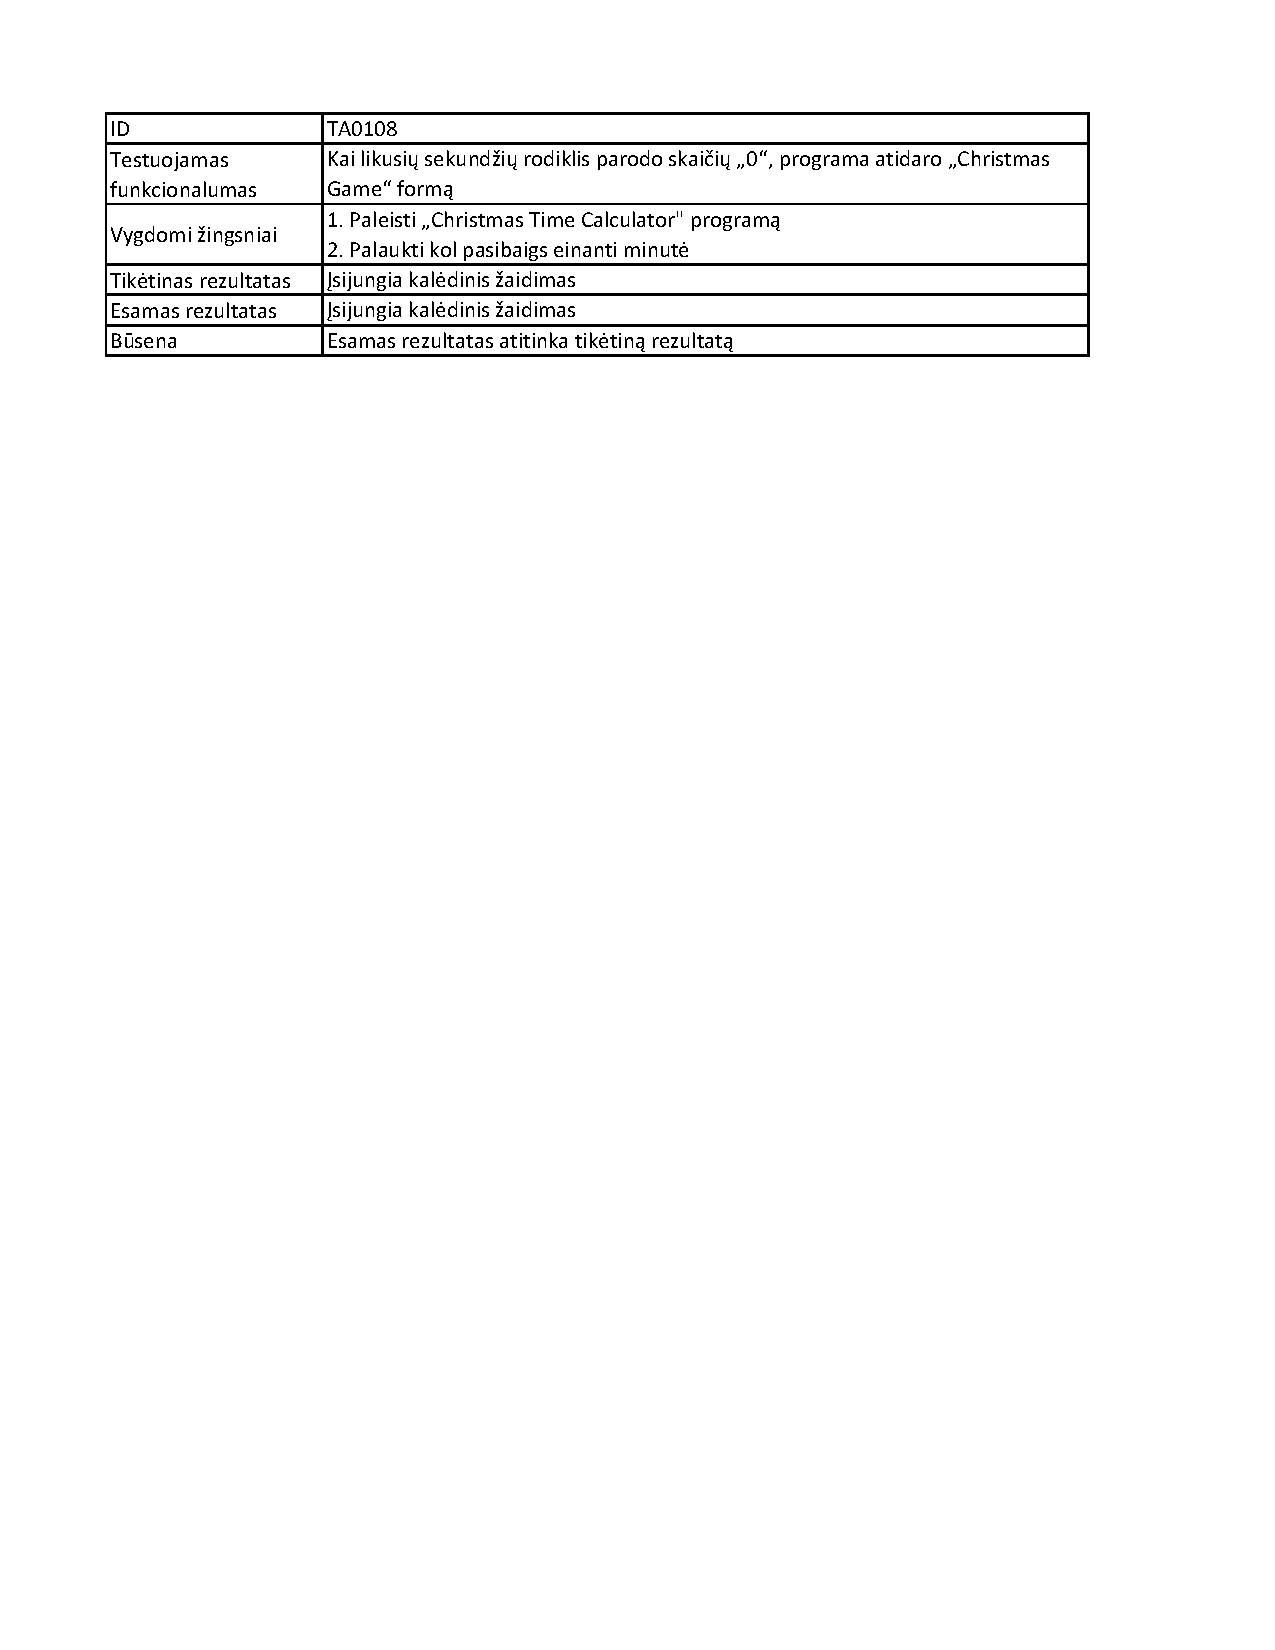
\includegraphics[width=\textwidth]{TA/TA0108}			
					\label{fig:TA0108}
				\end{table}
				\begin{table}[H]
					\centering
					\caption{Pagrindinio lango dydžio keitimo testavimo atvejis}
					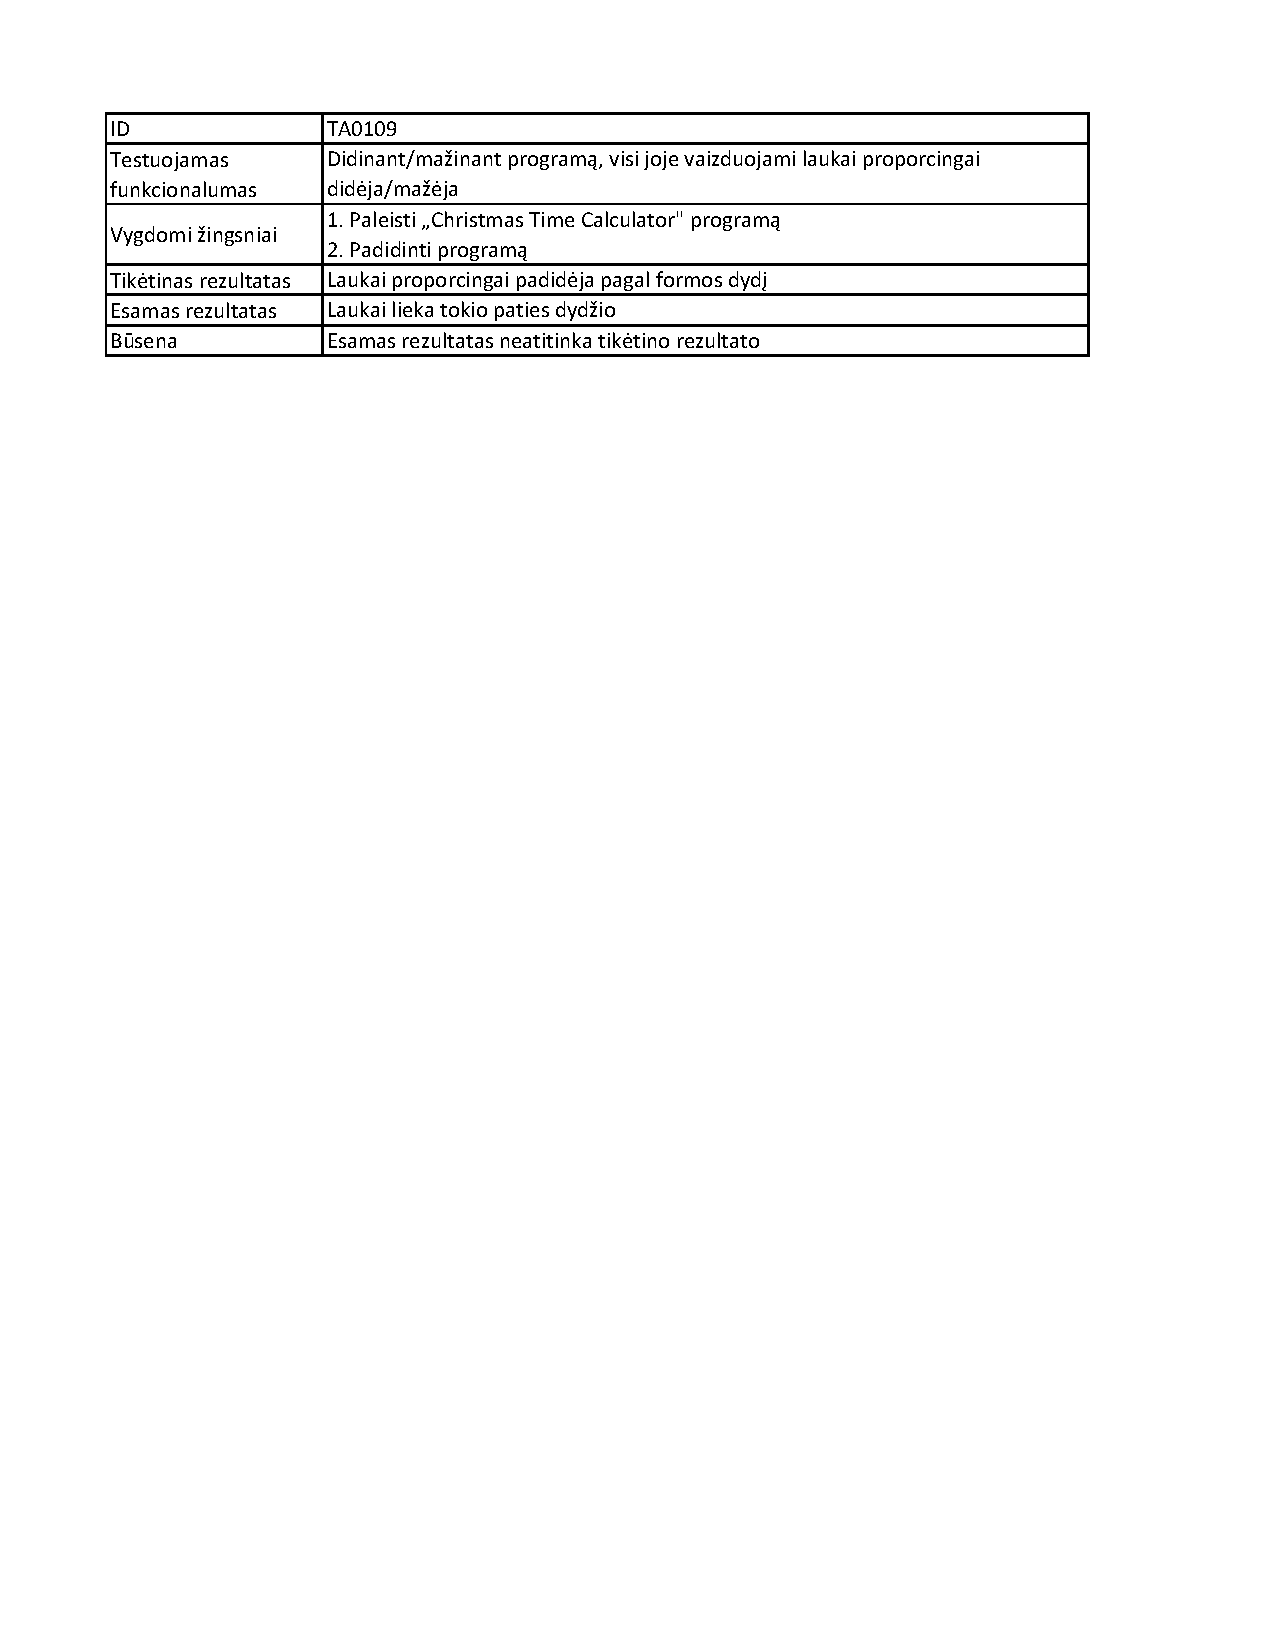
\includegraphics[width=\textwidth]{TA/TA0109}			
					\label{fig:TA0109}
				\end{table}
				\begin{table}[H]
					\centering
					\caption{Laiko pakartotinam žaidimo paleidimui testavimo atvejis}
					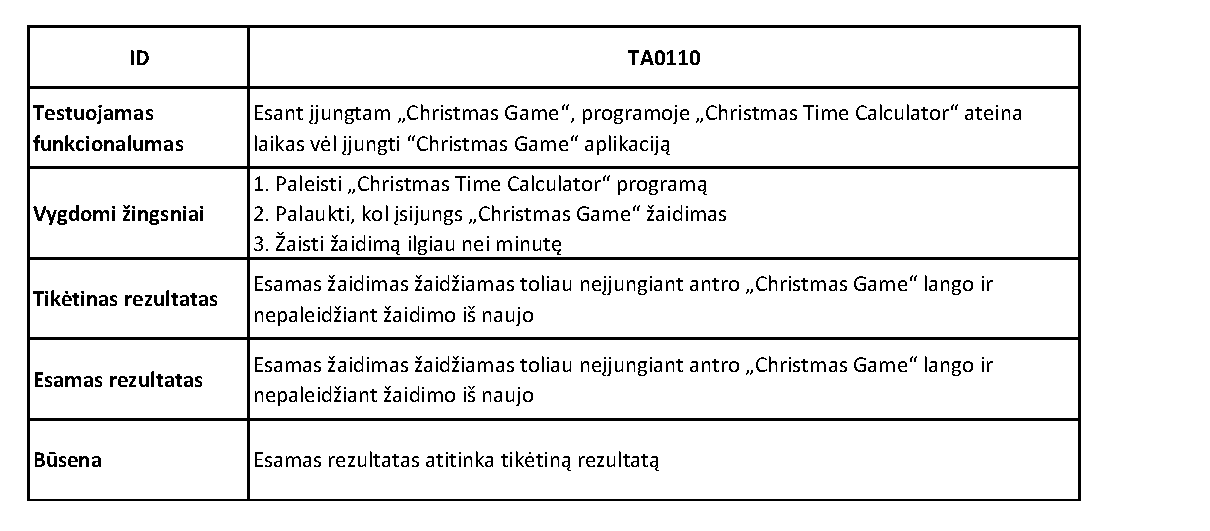
\includegraphics[width=\textwidth]{TA/TA0110}			
					\label{fig:TA0110}
				\end{table}
			\subsubsection{Papildomos dalies testavimo atvejai} \label{papildomosDaliesTA}
				Toliau 11 - 20 lentelėse pateikiami testavimo atvejai, apimantys papildomos dalies („Christmas Game“) funkcionalumą.
				\begin{table}[H]
					\centering
					\caption{Papildomo lango dydžio keitimo testavimo atvejis}
					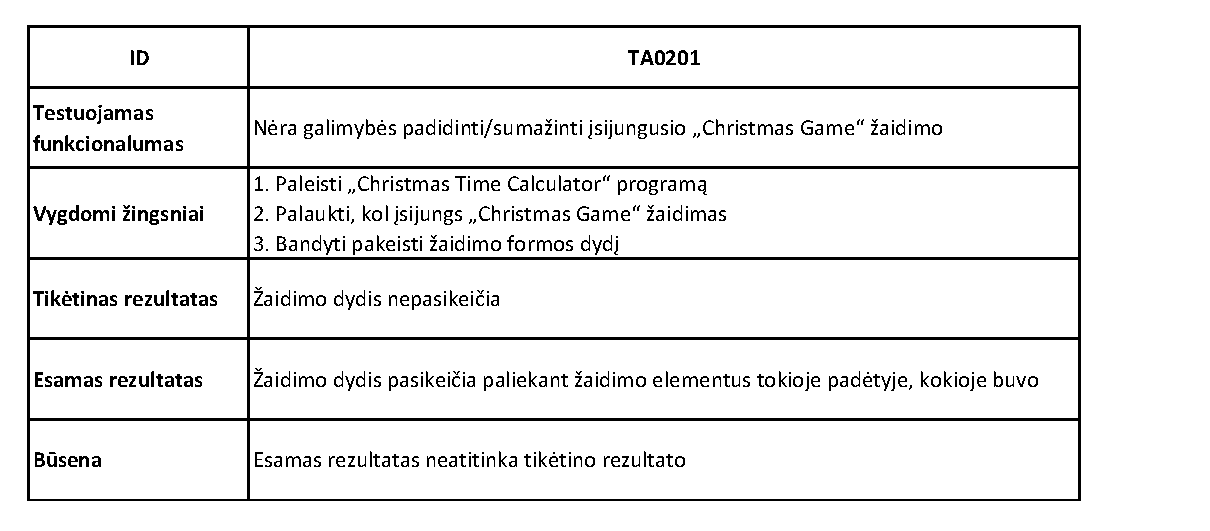
\includegraphics[width=\textwidth]{TA/TA0201}			
					\label{fig:TA0201}
				\end{table}
				\begin{table}[H]
					\centering
					\caption{„High Score“ laukelio testavimo atvejis}
					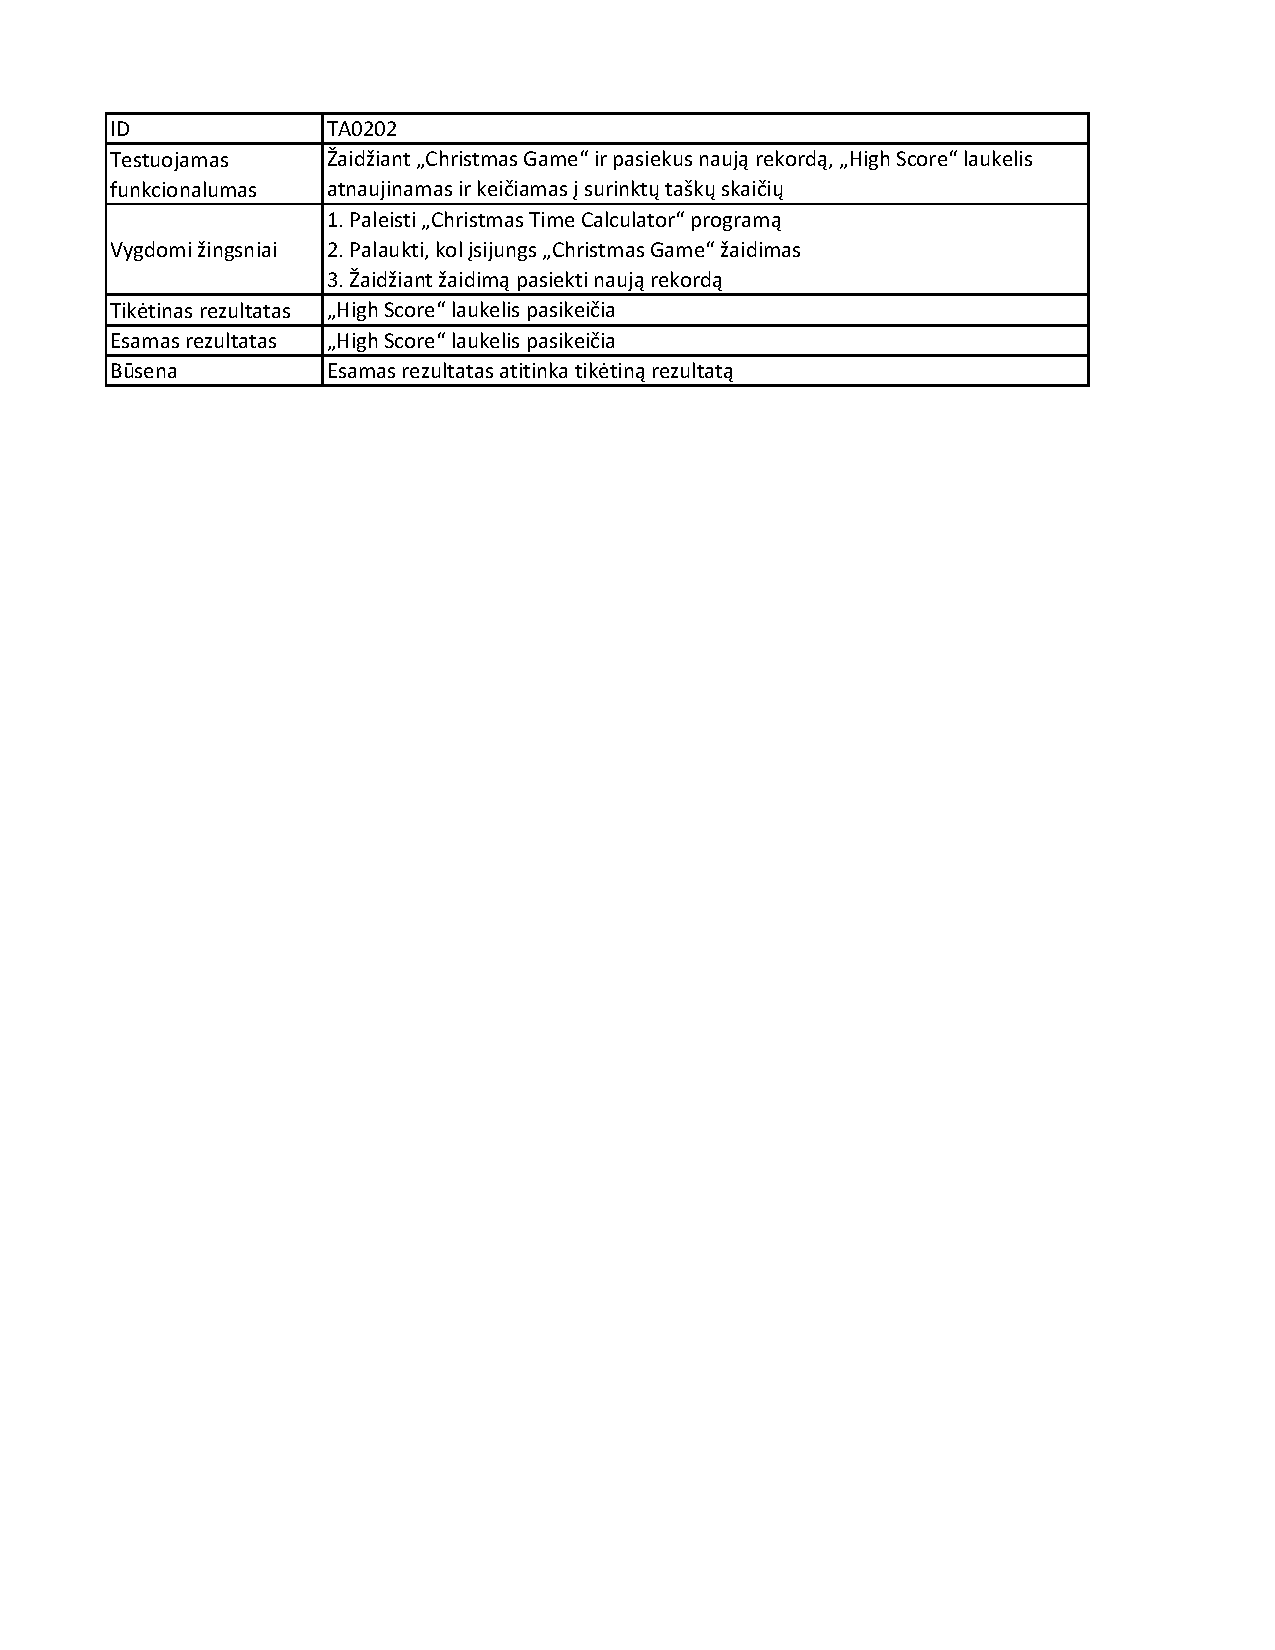
\includegraphics[width=\textwidth]{TA/TA0202}			
					\label{fig:TA0202}
				\end{table}
				\begin{table}[H]
					\centering
					\caption{Taškų skaičiavimo testavimo atvejis}
					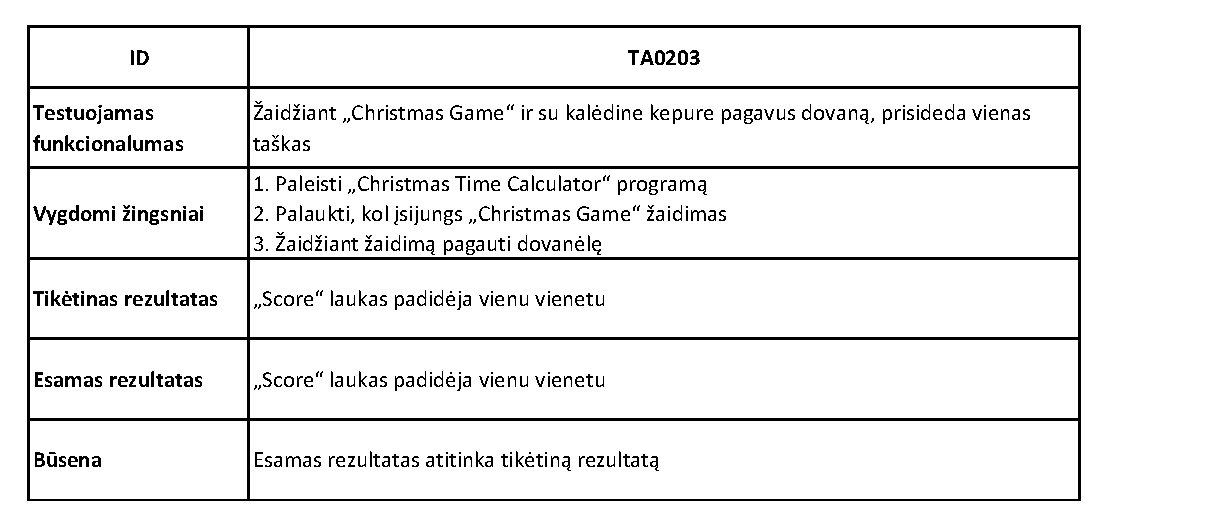
\includegraphics[width=\textwidth]{TA/TA0203}			
					\label{fig:TA0203}
				\end{table}
				\begin{table}[H]
					\centering
					\caption{Žaidimo valdymo testavimo atvejis}
					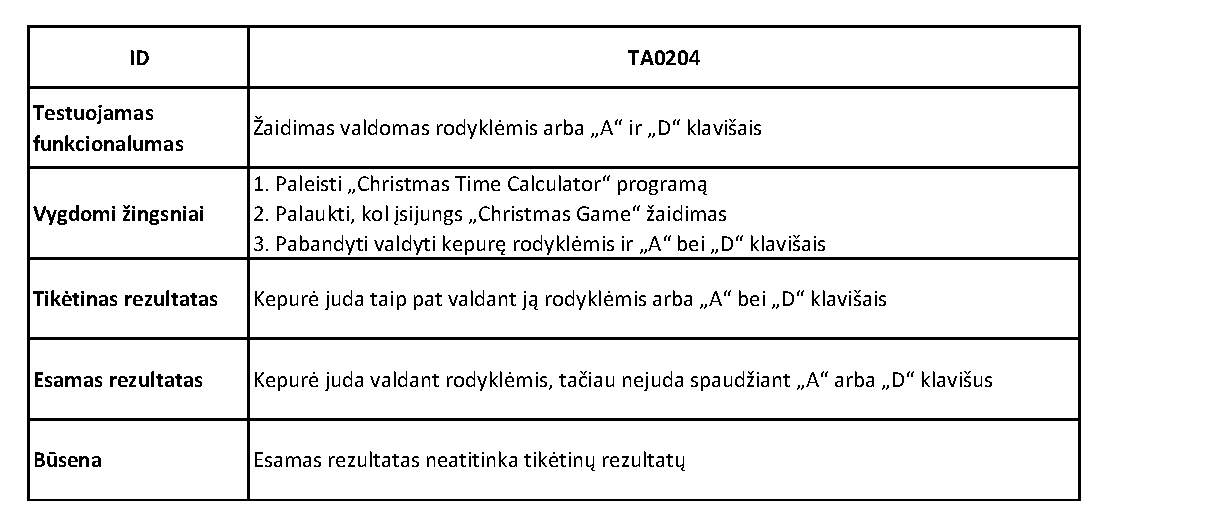
\includegraphics[width=\textwidth]{TA/TA0204}			
					\label{fig:TA0204}
				\end{table}
				\begin{table}[H]
					\centering
					\caption{Gyvybių skaičiavimo testavimo atvejis}
					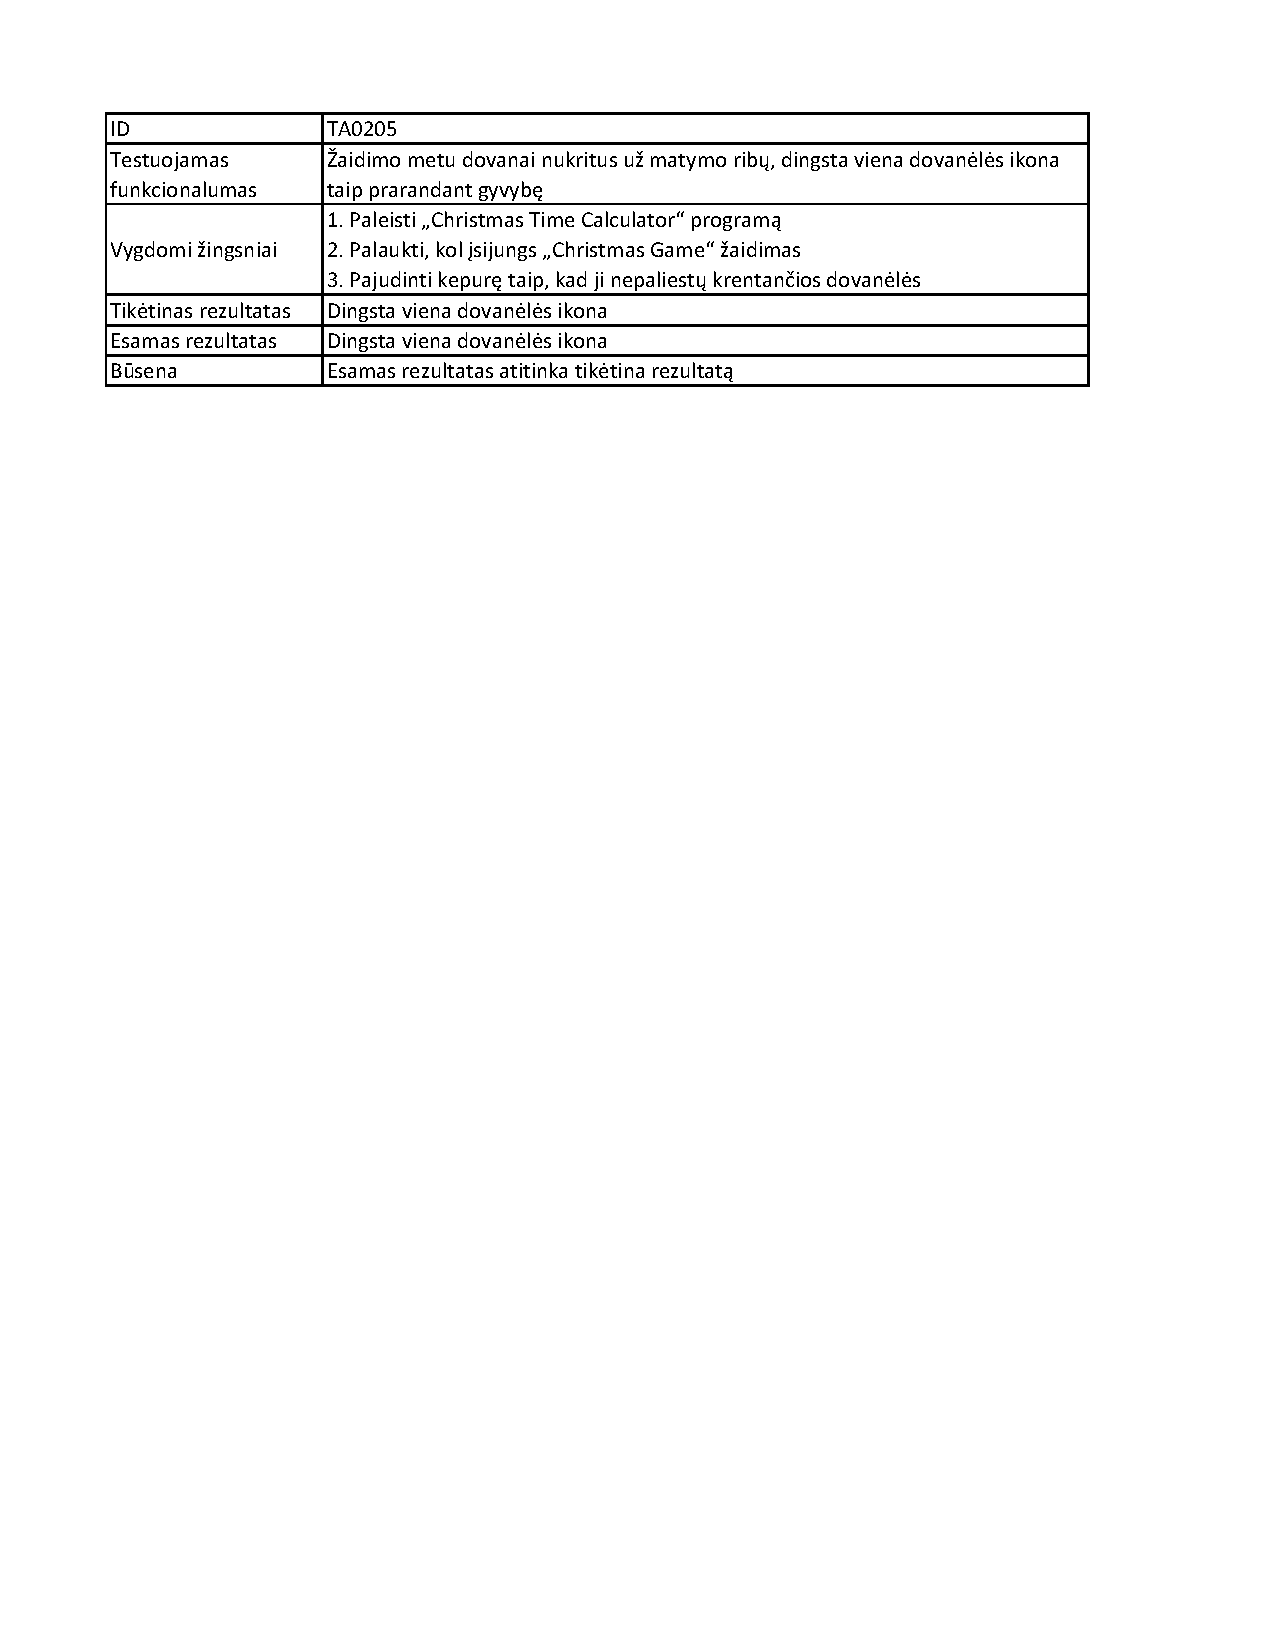
\includegraphics[width=\textwidth]{TA/TA0205}			
					\label{fig:TA0205}
				\end{table}
				\begin{table}[H]
					\centering
					\caption{Dovanėlių atvaizdavimo testavimo atvejis}
					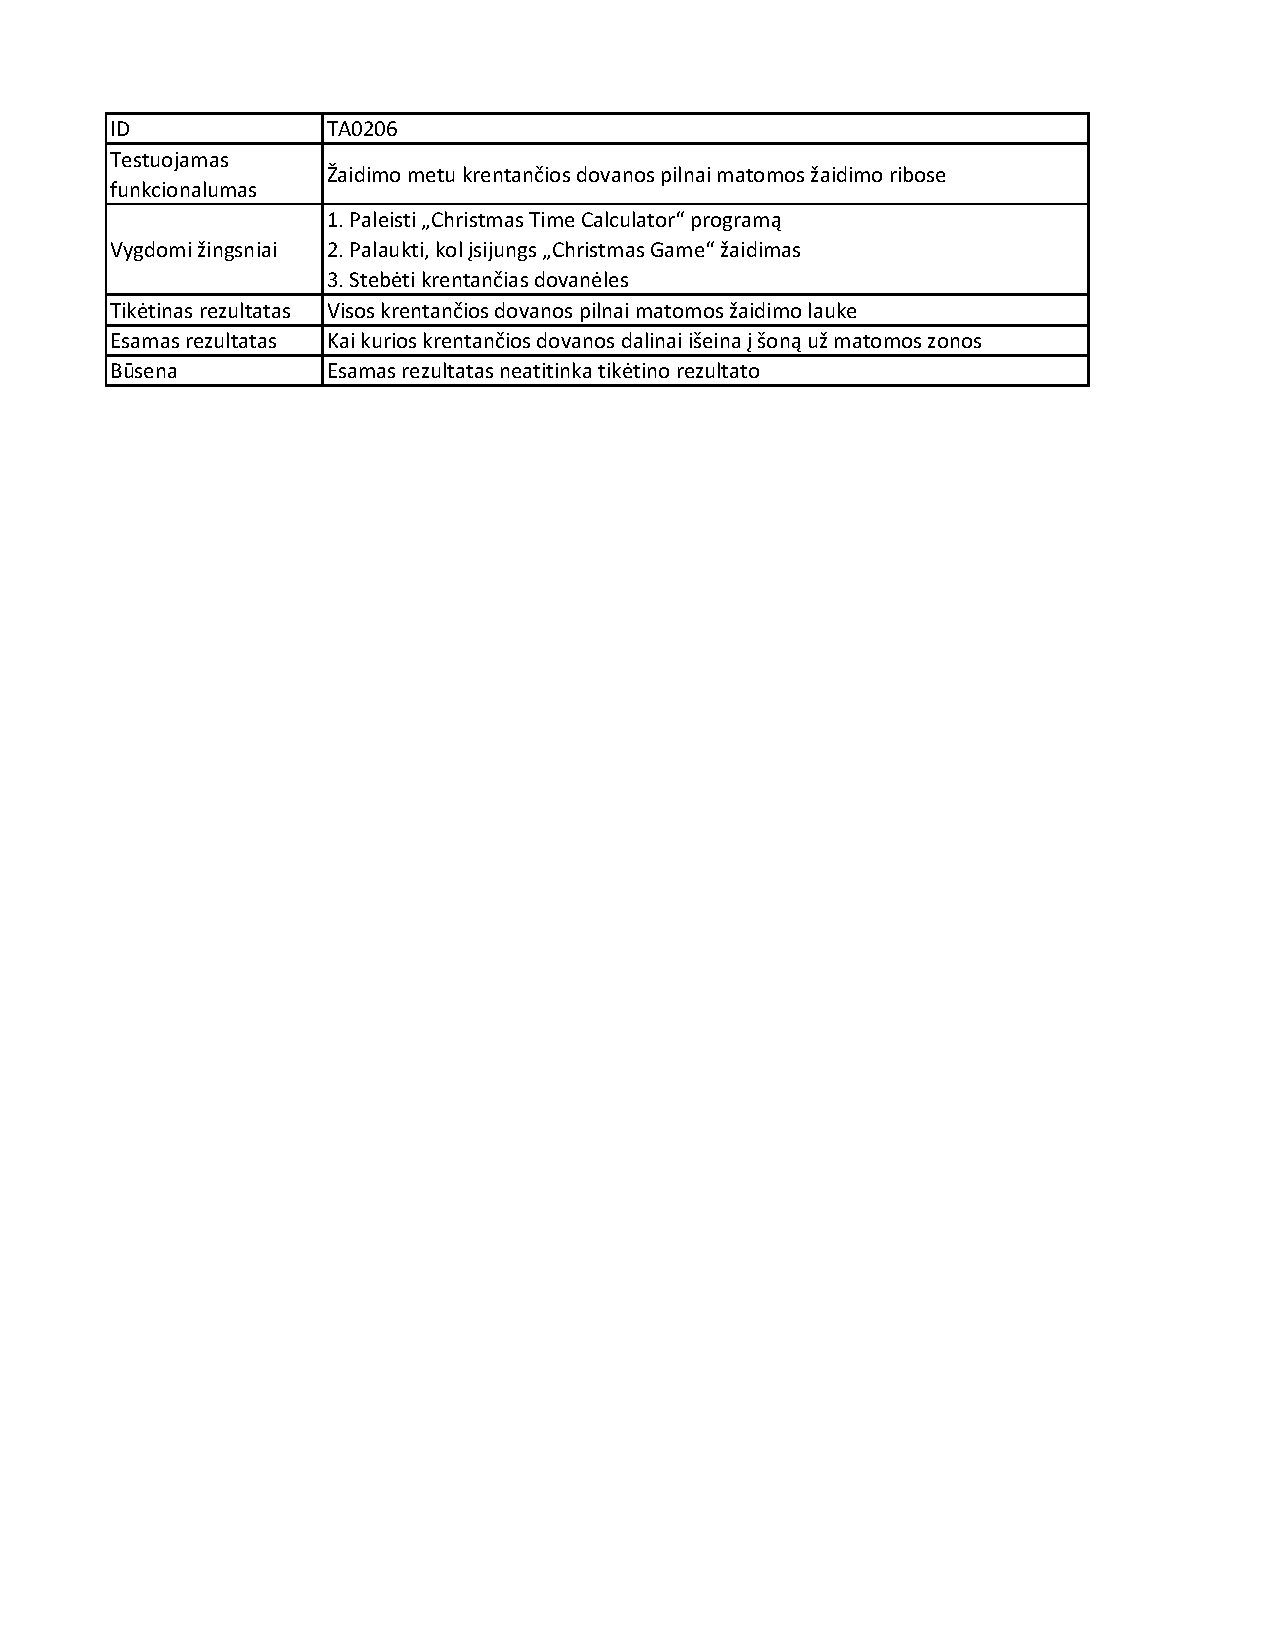
\includegraphics[width=\textwidth]{TA/TA0206}			
					\label{fig:TA0206}
				\end{table}
				\begin{table}[H]
					\centering
					\caption{Dovanėlių kritimo greičio didėjimo testavimo atvejis}
					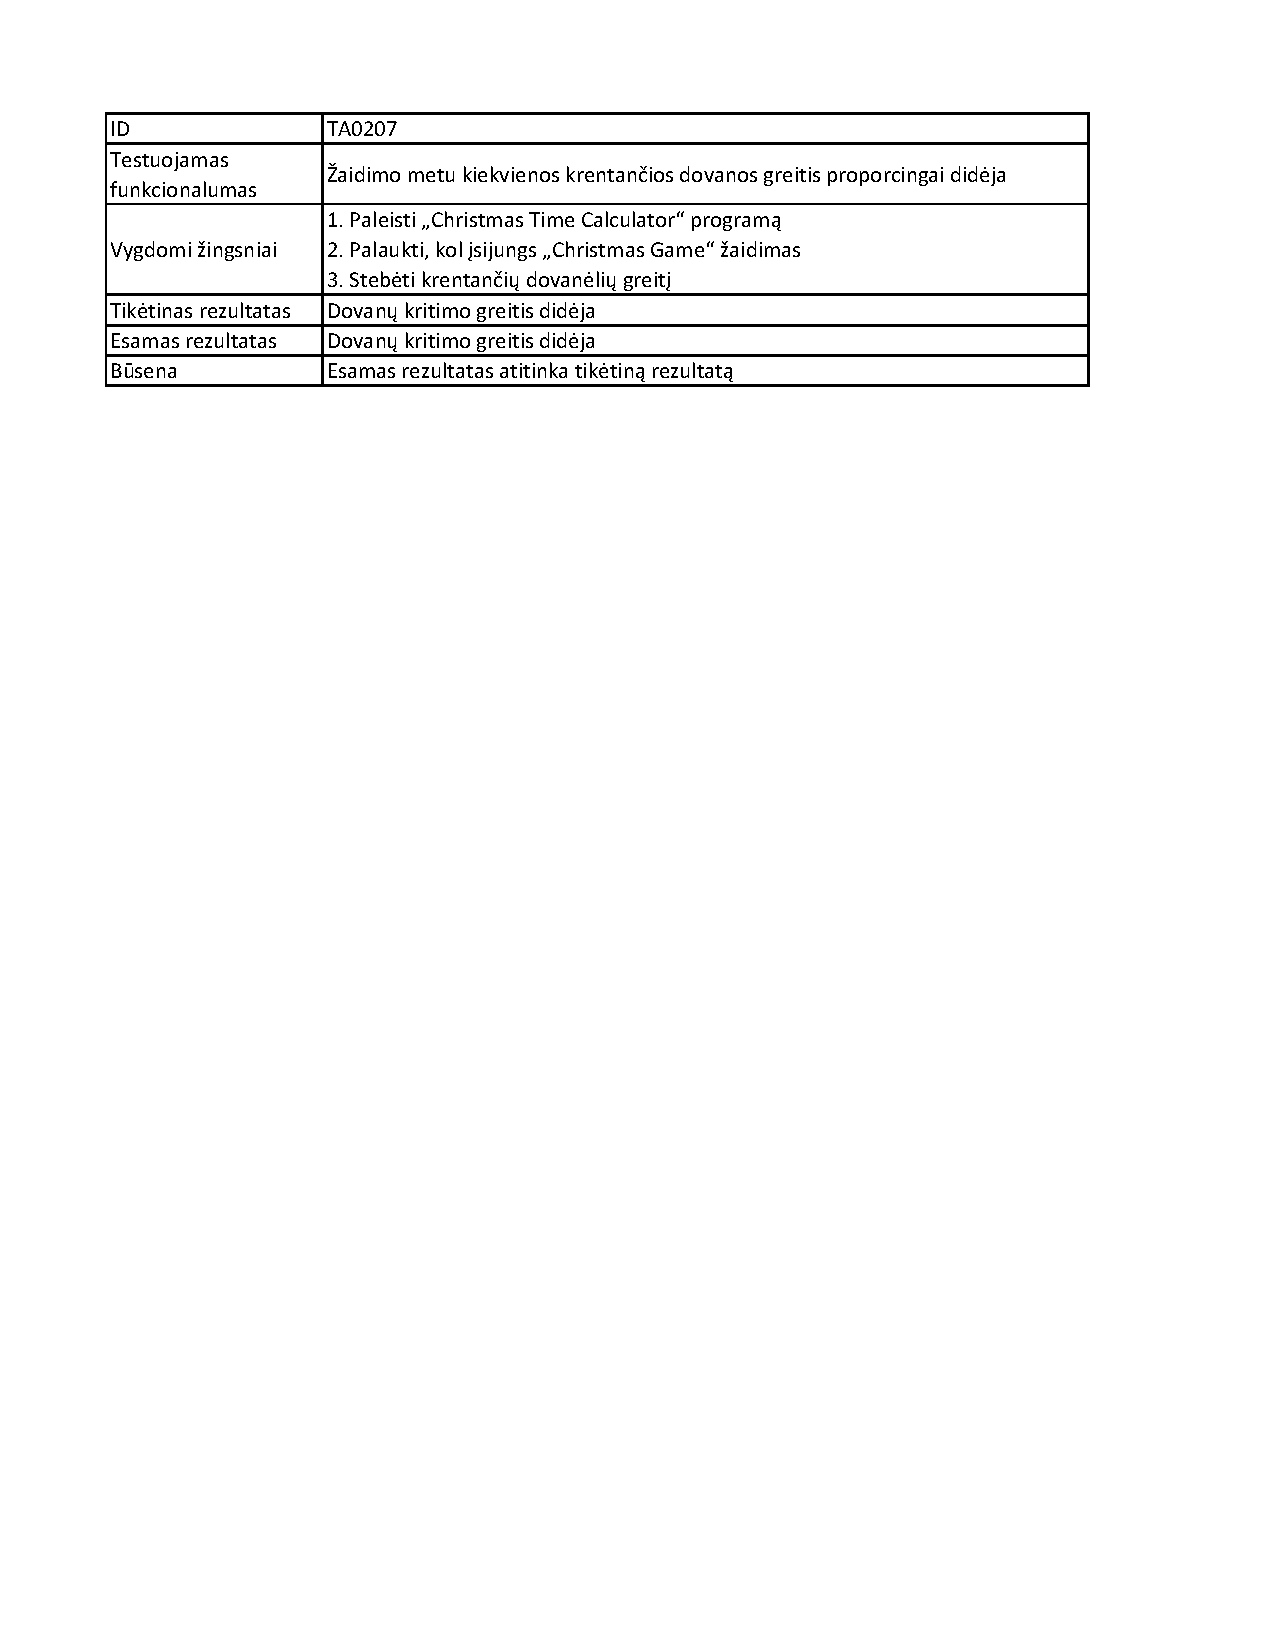
\includegraphics[width=\textwidth]{TA/TA0207}			
					\label{fig:TA0207}
				\end{table}
				\begin{table}[H]
					\centering
					\caption{Kalėdinės kepurėlės greičio didėjimo testavimo atvejis}
					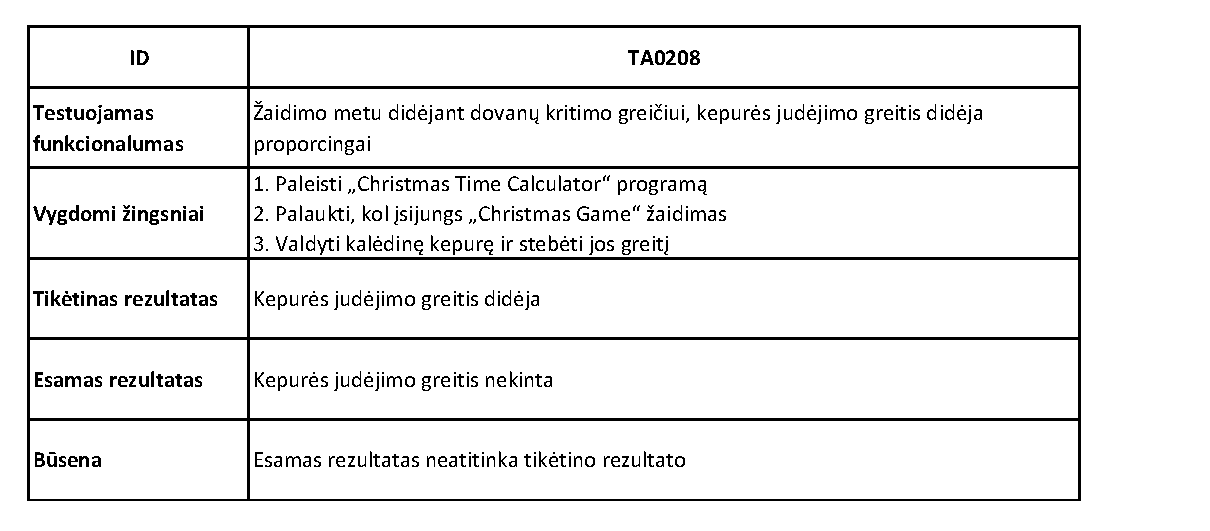
\includegraphics[width=\textwidth]{TA/TA0208}			
					\label{fig:TA0208}
				\end{table}
				\begin{table}[H]
					\centering
					\caption{Žaidimo pralaimėjimo be pasiekto rekordo testavimo atvejis}
					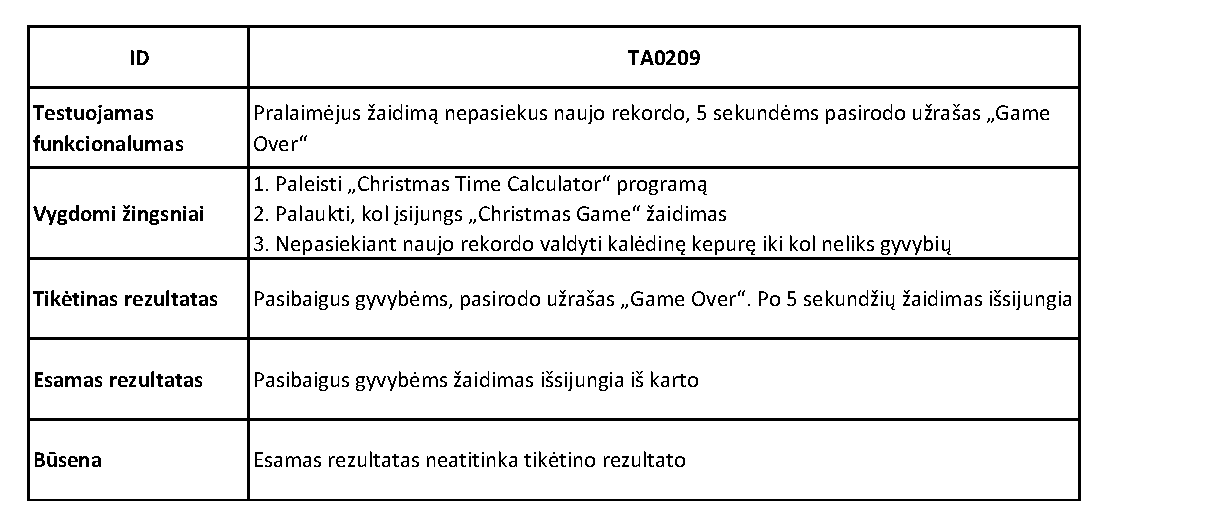
\includegraphics[width=\textwidth]{TA/TA0209}			
					\label{fig:TA0209}
				\end{table}
				\begin{table}[H]
					\centering
					\caption{Žaidimo pralaimėjimo su pasiektu rekordu testavimo atvejis}
					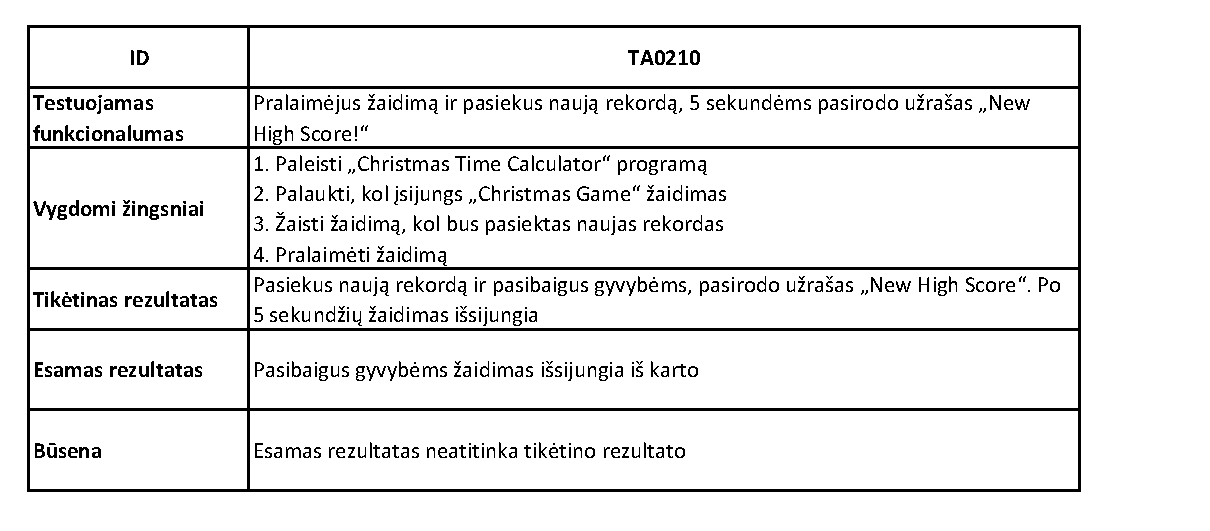
\includegraphics[width=\textwidth]{TA/TA0210}			
					\label{fig:TA0210}
				\end{table}
		\subsection{Reikalavimų - testavimo atvejų atsekamumo matrica} \label{atsekamumo matrica}
			Toliau 21 lentelėje pateikiama reikalavimų - testavimo atvejų atsekamumo matrica.
			\begin{table}[H]
				\centering
				\caption{Reikalavimų - testavimo atvejų atsekamumo matrica}
				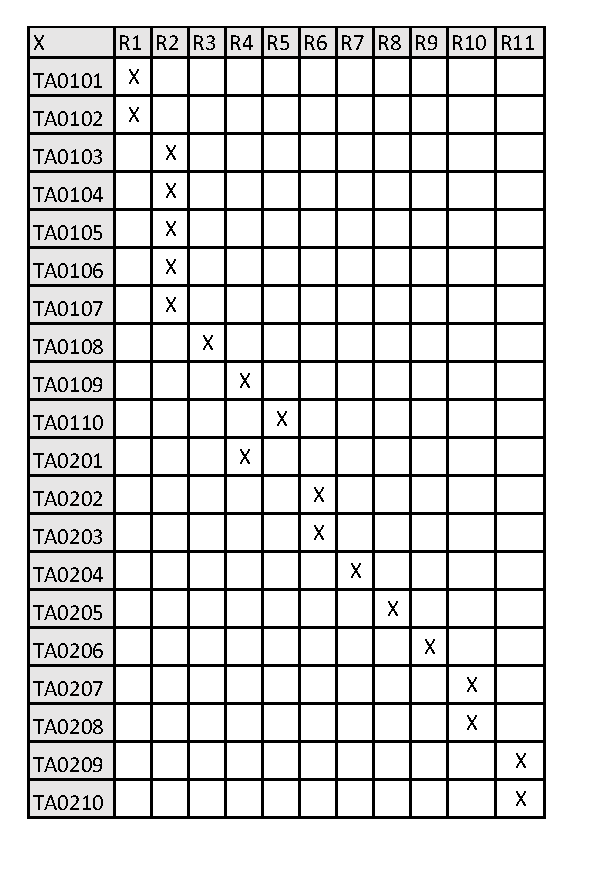
\includegraphics[width=\textwidth]{TA/AtsekamumoMatrica}			
				\label{fig:AtsekamumoMatrica}
			\end{table}
	\section{Defektų sąrašas} \label{defektai}
		Šiame skyriuje pateikiamas defektų sąrašas 22 lentelėje. Taip pat pateikiami defektų tipai:
			\begin{itemize}
				\item \textbf{Kritinis} - pažeistas pagrindinis funkcionalumas. 
				Defektą būtina taisyti prieš leidžiant šia programa naudotis kitiems.
				\item \textbf{Svarbus} - pažeistas šalutinis funkcionalumas. 
				Programa galima naudotis, tačiau šis funkcionalumas dalinai trikdys veiklą.
				\item \textbf{Neutralus} - kosmetinis ar mažai pastebimas defektas.
				Programa galima naudotis be pažeisto funkcionalumo.
			\end{itemize}
			\begin{table}[H]
				\centering
				\caption{Defektų sąrašas}
				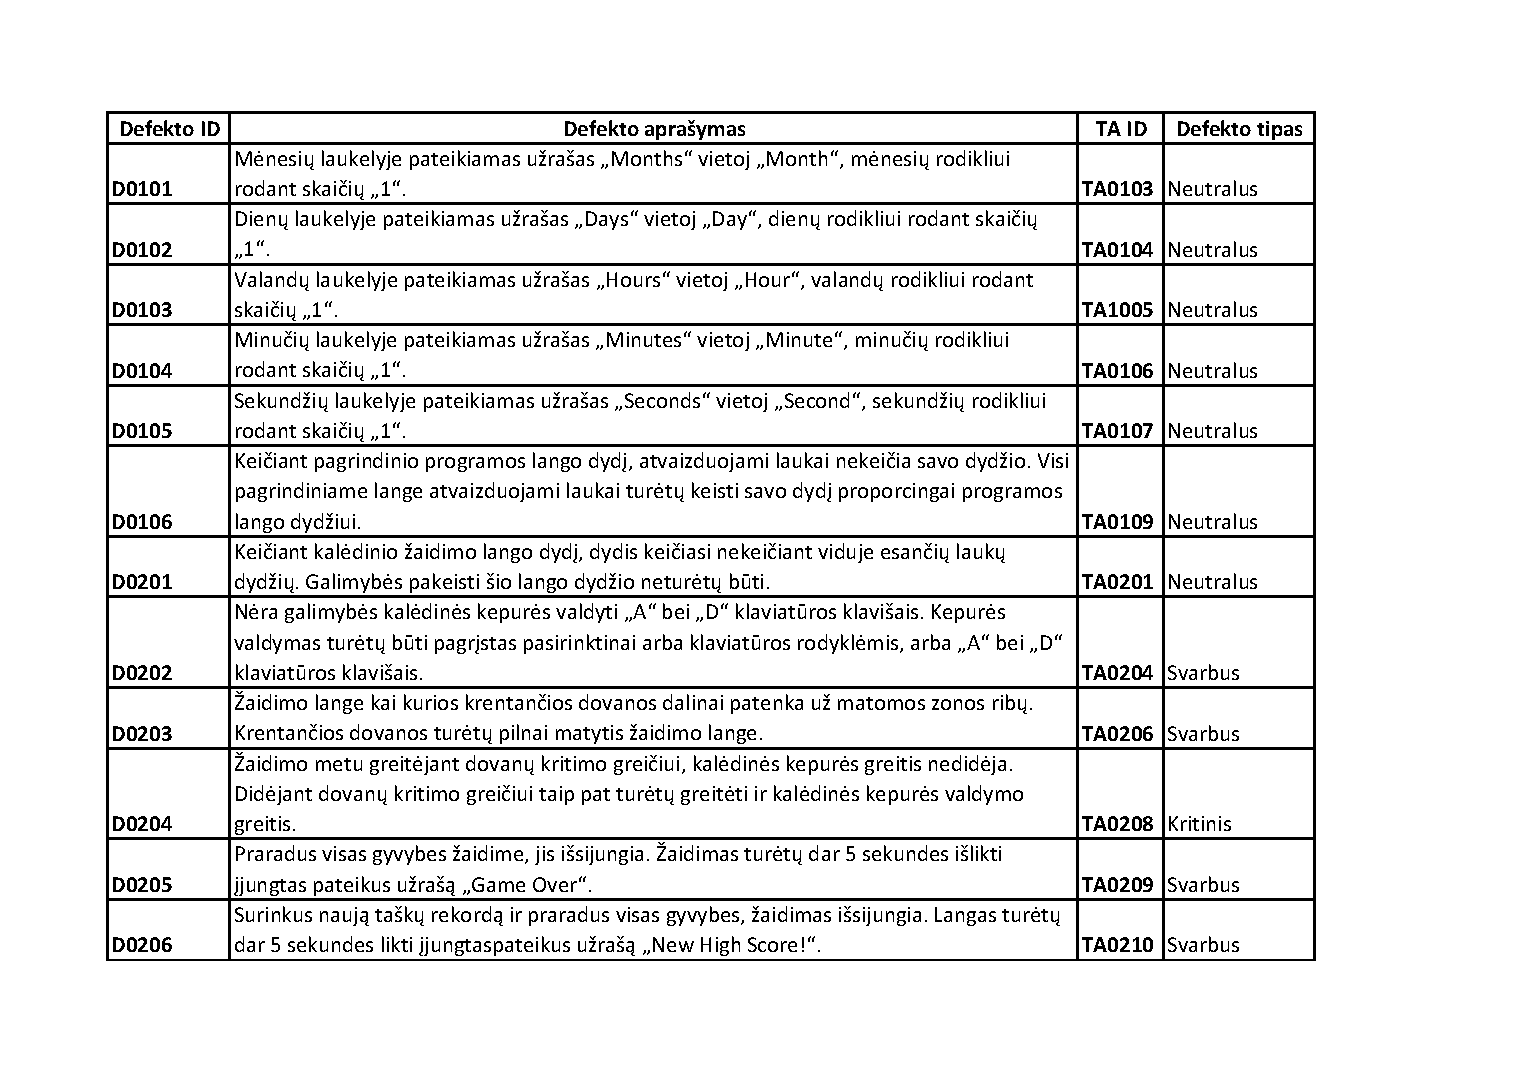
\includegraphics[width=\textwidth]{TA/Defektai}			
				\label{fig:DefektuSarasas}
			\end{table}
	\sectionnonum{Rezultatai} \label{rezultatai}
			Programos „Christmas Time Calculator“ testavimo metu buvo sudaryta 20 testavimo atvejų. 
			10 iš jų skirti pagrindinės programos dalies funkcionalumui patikrinti, kiti 10 - papildomos dalies, t. y. kalėdinio žaidimo
			funkcionalumui patikrinti.

			Pagrindinėje dalyje buvo aptikti šeši neutralūs defektai, nepažeidžiantys programos fukcionalumo.

			Papildomoje „Christmas Game“ dalyje buvo aptikti šeši defektai. Vienas iš jų neutralus, keturi svarbūs ir vienas kritinis.
	\sectionnonum{Išvados} \label{isvados}	
			
			Atlikus programos „Christmas Time Calculator“ testavimą paaiškėjo, kad pagrindinė šios programos dalies funkcionalumas 
			veikia su keliais neutraliais kosmetiniais defektais. Tačiau šia programa negalima leisti toliau naudotis kitiems asmenims,
			kol nebus ištaisytas kritinis defektas. Šis defektas neleidžia pilnai žaisti kalėdinio žaidimo, kadangi dovanoms krentant greičiau
			nėra galimybės jų pagauti su lėtai judančia kalėdine kepure. Taip pat norint, kad žaidimo eiga vyktų sklandžiau rekuomenduojama
			ištaisyti svarbius defektus.
	
	\sectionnonum{Priedai} \label{priedai}
		Šiame skyriuje pateikiami priedai, padedantys sklandžiau peržvelgti šį dokumentą.
		\subsection*{Terminų žodynėlis} \label{zodynas}
			\begin{itemize}
				\item \textbf{„Christmas Time Calculator“} - programa skaičiuojanti laiko likutį iki artimiausių Kalėdų, 
				pateikiant tikslų mėnesių, dienų, valandų, minučių ir sekundžių skaičių.
				\item \textbf{„Christmas Game“} - papildomas programos „Christmas Time Calculator“ langas, pasirodantis likus kiekvienai
				minutei mažiau iki Kalėdų (t. y. kai sekundžių rodiklis vaizduoja skaičių „0“). Šią dalį sudaro kalėdinis žaidimas,
				kurio veikimo principas yra valdant lango apačioje esančią kalėdinę kepurę surinkti kuo daugiau krentančių dovanų.
				\item \textbf{Pagrindinė dalis} - pirminis programos „Christmas Time Calculator“ langas.
				\item \textbf{Papildoma dalis} - „Christmas Game“ dalies langas.
				\item \textbf{Kalėdinis žaidimas} - žaidimas, atsiveriantis ikus kiekvienai minutei mažiau iki Kalėdų.
				\item \textbf{„High Score“ laukas} - papildomos dalies laukas, kuriame pateikiamas disžiausias žaidime surinktų taškų skaičius.
				\item \textbf{Kalėdinė kepurė} - kalėdinio žaidimo apačioje esanti į šonus valdoma kalėdinės kepurės formos ikona.
				\item \textbf{Dovana} - kalėdiniame žaidime krentantčios ikonos, kurias palietus su kalėdine kepure pridedamas vienas taškas
				ir jai nukrentant už ribų panaikinama viena gyvybė. 
			\end{itemize}
\end{document}
